\newcommand{\NWtarget}[2]{\hypertarget{#1}{#2}}
\newcommand{\NWlink}[2]{\hyperlink{#1}{#2}}
\newcommand{\NWtxtMacroDefBy}{Fragment defined by}
\newcommand{\NWtxtMacroRefIn}{Fragment referenced in}
\newcommand{\NWtxtMacroNoRef}{Fragment never referenced}
\newcommand{\NWtxtDefBy}{Defined by}
\newcommand{\NWtxtRefIn}{Referenced in}
\newcommand{\NWtxtNoRef}{Not referenced}
\newcommand{\NWtxtFileDefBy}{File defined by}
\newcommand{\NWtxtIdentsUsed}{Uses:}
\newcommand{\NWtxtIdentsNotUsed}{Never used}
\newcommand{\NWtxtIdentsDefed}{Defines:}
\newcommand{\NWsep}{${\diamond}$}
\newcommand{\NWnotglobal}{(not defined globally)}
\newcommand{\NWuseHyperlinks}{}
\documentclass[10pt, english, oneside]{report}
\usepackage[a4paper, left=1cm, right=1cm, top=3cm, marginparwidth=2cm]{geometry}
\usepackage{marginnote}

\setcounter{secnumdepth}{3} % default value for 'report' class is "2"


\usepackage[utf8]{inputenc}
\usepackage[T1]{fontenc}
\usepackage{tikzsymbols}
\usepackage[backend=bibtex, style=numeric, sorting=none]{biblatex} 
\usepackage{csquotes}
\setlength\bibitemsep{\baselineskip}
\addbibresource{References.bib}

\usepackage{float} % to take away the error unknown float option `H'
% https://stackoverflow.com/a/27243065/505306
% Making caption font smaller on figures and tables.
\usepackage{caption}
\captionsetup{font=footnotesize}

%-------------------------------------------------------------------------------
%\usepackage[left,pagewise]{lineno}
%\usepackage[right]{lineno}
%\linenumbers
%--------------------------------------------------------------------------------
\usepackage[framemethod=TikZ]{mdframed}
\usepackage{wrapfig}
\usepackage{amsthm}
\usepackage{amsfonts}
% ------------------------------------------------------------------------------
\usepackage[toc,page]{appendix}
\usepackage[stretch=10]{microtype} % https://tex.stackexchange.com/a/586  The great microtype package
%-------------------------------------------------------------------------------
%https://tex.stackexchange.com/a/278199/17858
% For aligning itemize environments to left
\usepackage{enumitem}
\mdfsetup{%
   middlelinecolor=red,
   middlelinewidth=0pt,
   roundcorner=10pt}

\mdfdefinestyle{MyFrame}{%
    linecolor=black,
    outerlinewidth=0.1pt,
    roundcorner=0pt,
    innertopmargin=14pt,
    innerbottommargin=4pt,
    innerrightmargin=4pt,
    innerleftmargin=4pt,
        leftmargin = 4pt,
        rightmargin = 4pt,
    %backgroundcolor=gray!50!white}
     }
%-------------------------------------------------------------------------------

\definecolor{theocol}{RGB}{255, 222, 228}
\newtheorem{theo}{Theorem}
\newenvironment{ftheo}
  {\begin{mdframed}[style=MyFrame,nobreak=true, backgroundcolor=theocol]\begin{theo}}
  {\end{theo}\end{mdframed}}


\definecolor{lemcol}{RGB}{226, 255, 220}
\newtheorem{lem}{Lemma}
\newenvironment{flem}
  {\begin{mdframed}[style=MyFrame,nobreak=true, backgroundcolor=lemcol]\begin{lem}}
  {\end{lem}\end{mdframed}}

\definecolor{corcol}{RGB}{227, 227, 227}
\newtheorem{cor}{Corollary}
\newenvironment{fcor}
  {\begin{mdframed}[style=MyFrame,nobreak=true, backgroundcolor=corcol]\begin{cor}}
  {\end{cor}\end{mdframed}}

\definecolor{propcol}{RGB}{227, 227, 227}
\newtheorem{prop}{Proposition}
\newenvironment{fprop}
  {\begin{mdframed}[style=MyFrame,nobreak=true, backgroundcolor=propcol]\begin{prop}}
  {\end{prop}\end{mdframed}}

\definecolor{conjcol}{RGB}{248, 218, 194}
\newtheorem{conj}{Conjecture}
\newenvironment{fconj}
  {\begin{mdframed}[style=MyFrame,nobreak=true, backgroundcolor=conjcol]\begin{conj}}
  {\end{conj}\end{mdframed}}


\definecolor{notecol}{RGB}{255, 152, 149  }
\newenvironment{note}
  {\begin{mdframed}[style=MyFrame,nobreak=true, backgroundcolor=notecol]}
  {\end{mdframed}}

\usepackage{enumitem}

%-------------------------------------------------------------------------------
% https://tex.stackexchange.com/q/2291/17858
% if you want to create a new list from scratch
\newlist{alphalist}{enumerate}{1}
% in that case, at least label must be specified using \setlist
\setlist[alphalist,1]{label=\textbf{\Alph*.}}

%--------------------------------------------------------------------------------
\usepackage[english]{babel}
%\setlength{\voffset}{-0.75in}
\setlength{\headsep}{5pt}

%-------------------------------------------------------------------------------
\usepackage{blindtext}
\usepackage{lipsum}
\usepackage{kantlipsum}
\usepackage{textcomp}

\usepackage{amssymb}
\usepackage{amsmath}
\usepackage{IEEEtrantools}
\usepackage{mathtools}

\usepackage{listings}


%-----------------------------------------------------------------------------------------------
\usepackage[inline]{asymptote}
\usepackage{asypictureB}
\usepackage{filecontents}
\usepackage{parskip} 
\usepackage{tocloft}
\usepackage{graphicx}                             % Include images into pdf document 
\usepackage{tikz}                                 % Useful for the circled command. Don't remove!
\usepackage{multicol}                             % For lists in two or more columns


%% top right numbering of pages https://tex.stackexchange.com/a/56321
\pagestyle{myheadings}



\usepackage[nokwfunc, ruled, linesnumbered,nofillcomment]{algorithm2e}
\newcommand\mycommfont[1]{\footnotesize\ttfamily\textcolor{gray}{#1}}
\SetCommentSty{mycommfont}

\usepackage[T1]{fontenc}
%------------------------------------------------------------------------------------------------
\usepackage{needspace}                % So that sections/code-blocks don't straddle two pages 
\usepackage{mathtools}
\usepackage{subfig}
\usepackage{etoolbox}
\usepackage{color}
\usepackage{pifont}
\setlength{\parindent}{20pt}
% For italicizing quotes: https://tex.stackexchange.com/a/288556/17858

%------------------------------------------------------------------------------------------------
\usepackage{quoting,xparse}  %%% from https://tex.stackexchange.com/a/391739

\NewDocumentCommand{\bywhom}{m}{% the Bourbaki trick
  {\nobreak\hfill\penalty50\hskip1em\null\nobreak
   \hfill\mbox{\normalfont(#1)}%
   \parfillskip=0pt \finalhyphendemerits=0 \par}%
}

\NewDocumentEnvironment{pquotation}{m}
  {\begin{quoting}[
     indentfirst=true,
     leftmargin=\parindent,
     rightmargin=\parindent]\itshape}
  {\bywhom{#1}\end{quoting}}


%------------------------------------------------------------------------------------------------
% Convenience commands
\newcommand*\circled[1]{\tikz[baseline=(char.base)]{\node[shape=circle,draw,inner sep=2pt] (char) {#1};}}
\providecommand{\myceil}[1]{\left \lceil #1 \right \rceil }	% Ceil function
\providecommand{\myfloor}[1]{\left \lfloor #1 \right \rfloor }	% Floor function\renewcommand{\labelitemi}{\tiny$\blacksquare$}	
\newcommand\given[1][]{\:#1\vert\:}                             % for drawing the conditional probability `|` sign neatly.
\newcommand\RR{\mathbb{R}}					% Set of reals numbers
\newcommand\CC{\mathbb{C}}					% Set of complex numbers
\newcommand\ZZ{\mathbb{Z}}					% Set of integers
\newcommand\NN{\mathbb{N}}					% Set of naturals
\newcommand\rarr{\rightarrow}					% Rightarrow
\newcommand\larr{\leftarrow}					% Leftarrow
\newcommand\defeq{\coloneqq}					% := symbol
\renewcommand\tilde{ \: \thicksim \: }				% Sane tildas

\newmdenv[topline=false, bottomline=false, skipabove=\topsep,skipbelow=\topsep]{siderules}

% https://tex.stackexchange.com/a/458876/17858 rounded
% pink rectangles around an inline word
\newcommand{\sticker}[1]{\tikz[baseline=(X.base)]\node [draw=red,fill=pink!60,semithick,
     rectangle,inner sep=2pt, rounded corners=3pt] (X) { {\footnotesize \color{red} #1}};}

\newif\ifshowcode
\showcodetrue
\usepackage{latexsym}
\usepackage{listings}
\usepackage{color}
\definecolor{linkcolor}{rgb}{0.7, 0, 0}

\usepackage{todonotes}
\usepackage{booktabs}

\usepackage[%
raiselinks,%
pdfhighlight=/O,%
hyperfigures,%
breaklinks,%
colorlinks,%
pdfstartview=FitBH,%
linkcolor={linkcolor},%
anchorcolor={linkcolor},%
citecolor={linkcolor},%
filecolor={linkcolor},%
menucolor={linkcolor},%
urlcolor={linkcolor}%
]{hyperref}

% taken from https://tex.stackexchange.com/a/371469 
% fior drawing a nice rule across the page
\newcommand\myrule{\par\noindent\rule{\textwidth}{0.4pt}}

%---------------------------------------------------------
\usepackage{xcolor}
\usepackage{sectsty}
\allsectionsfont{\sffamily}
\definecolor{lava}{rgb}{0.81, 0.06, 0.13}
\definecolor{mahogany}{rgb}{0.75, 0.25, 0.0}
\definecolor{sacramentostategreen}{rgb}{0.0, 0.34, 0.25}
%---------------------------------------------------------


%-------------------------------------
%\usepackage[toc]{multitoc}
%\renewcommand*{\multicolumntoc}{2}
%\setlength{\columnsep}{1cm}
%\setlength{\columnseprule}{0.1pt} % for a vertical separator between the columns
%------------------------------------

\setcounter{tocdepth}{2}

%-----------------------------------------------------------------------------------------
% FOR SOURCE CODE FORMATTING
\definecolor{cosmiclatte}{rgb}{1.0, 0.97, 0.91}
\definecolor{asparagus}{rgb}{0.53, 0.66, 0.42}
\lstdefinestyle{numbers} {numbers=left, stepnumber=1, numberstyle=\tiny, numbersep=10pt}
\lstdefinestyle{MyFrame}{backgroundcolor=\color{cosmiclatte},frame=shadowbox}

\lstdefinestyle{MyPythonStyle} {language=Python,style=MyFrame,frame=lines}
\lstset{language=Python,
                basicstyle=\ttfamily,
                keywordstyle=\color{blue}\ttfamily,
                stringstyle=\color{red}\ttfamily,
                commentstyle=\color{asparagus}\ttfamily,
                morecomment=[l][\color{magenta}]{\#}}


\lstdefinestyle{MyHaskellStyle} {language=Haskell,style=MyFrame,frame=lines}
\lstset{language=Haskell,
                basicstyle=\ttfamily,
                keywordstyle=\color{blue}\ttfamily,
                stringstyle=\color{red}\ttfamily,
                commentstyle=\color{asparagus}\ttfamily,
                morecomment=[l][\color{magenta}]{\#}}
%-----------------------------------------------------------------------------------------
\usepackage{marginnote}

\newcommand\margin[1]{\marginnote{\color{cadmiumgreen}{#1} }}				% Sane tildas
\definecolor{cadmiumgreen}{rgb}{0.0, 0.42, 0.24}
%---------------------------------------------------------------------------------------------------
\renewcommand{\labelitemi}{\scriptsize$\blacksquare$} % squaremarkers for bullets of itemized lists


%-------------------------------------------------------------------------------
% To express an idea in a crunchy way.
\newcommand{\crunchy}[1]{\lbrack{} \large \textit{#1} \normalsize \rbrack} 



% For italicizing quotes https://tex.stackexchange.com/a/288556
\usepackage{csquotes}
\renewcommand{\mkbegdispquote}[2]{\itshape}

% for italcizing figure captions
\usepackage[font={small,it}]{caption} % from https://tex.stackexchange.com/a/832


\SetKwComment{Comment}{$\triangleright$\ }{}
\newcommand{\myblue}[1]{{\color{blue}{#1}}}

\newcommand{\tss}{\textsuperscript}

\title{\huge{\bfseries{Coordinating Heterogenous Agents for Fast Package Delivery --- The Package Handoff Problem}}}
\author{Jie Gao $^1$, 
       Kien Huynh $^1$, 
       Joseph S. B. Mitchell $^2$, 
       Gaurish Telang$^2$}
\date{
\small{$^1$ Department of Computer Science, Stony Brook University \\%
$^2$ Department of Applied Mathematics and Statistics, Stony Brook University} \\[2ex]% 
}

\begin{document}
\maketitle

\begin{abstract}
How do you get a package from an initial location $S$ to a destination point $T$ using a 
fleet of ``heterogenous'' carrier agents (e.g. drones, taxis). By ``heterogenous'' we mean 
the two agents can have different capabilities like different maximum speed
or different fuel capacity. 

\vspace{2mm}

In the simplest version of the category of problems, 
we are given as input the initial locations of $n$  agents in $\mathbb{R}^2$ 
each capable of a maximum speed $u_i >0$ (where $u_i$ need \textsl{not} be equal to $v_j$ for $i \neq j$). 
Each agent can pick up the package and move to another point to \textit{rendezvous with} \underline{and} 
\textit{hand off} the 
package to another agent. This other agent then either proceeds to $T$ or decides to meet with 
and hand off the package to another agent, until the last agent decides to head directly to $T$. 

\vspace{2mm}

The objective is to get the agents to cooperate to send the package from $S$ to $T$ in the 
least possible time. We call this the \textit{Package Handoff Problem}. 

\vspace{2mm}

To solve this problem and its various avatars we need to 

\vspace{2mm}

\begin{enumerate}
\item Figure out which subset $S = \{i_1, i_2, \ldots i_k\}$ of the drones are used in the optimal schedule. 
\item Find the order in which the handoffs happend between the drones used in a schedule. 
\item Calculate the ``handoff'' points where drone $i_m$ hands over the package to drone 
      $i_{m+1}$, for $1 \leq m \leq k-1$
\end{enumerate}

\vspace{2mm}

This report is an algorithmic study of various heuristics developed to solve different variants of Package Handoff.

\end{abstract}


\newpage
\setcounter{tocdepth}{2}
\tableofcontents

%--------------------------
\chapter{Single Package Handoff}

\section{Introduction}
\begin{wrapfigure}{R}{0.5\textwidth}
  \begin{center}
    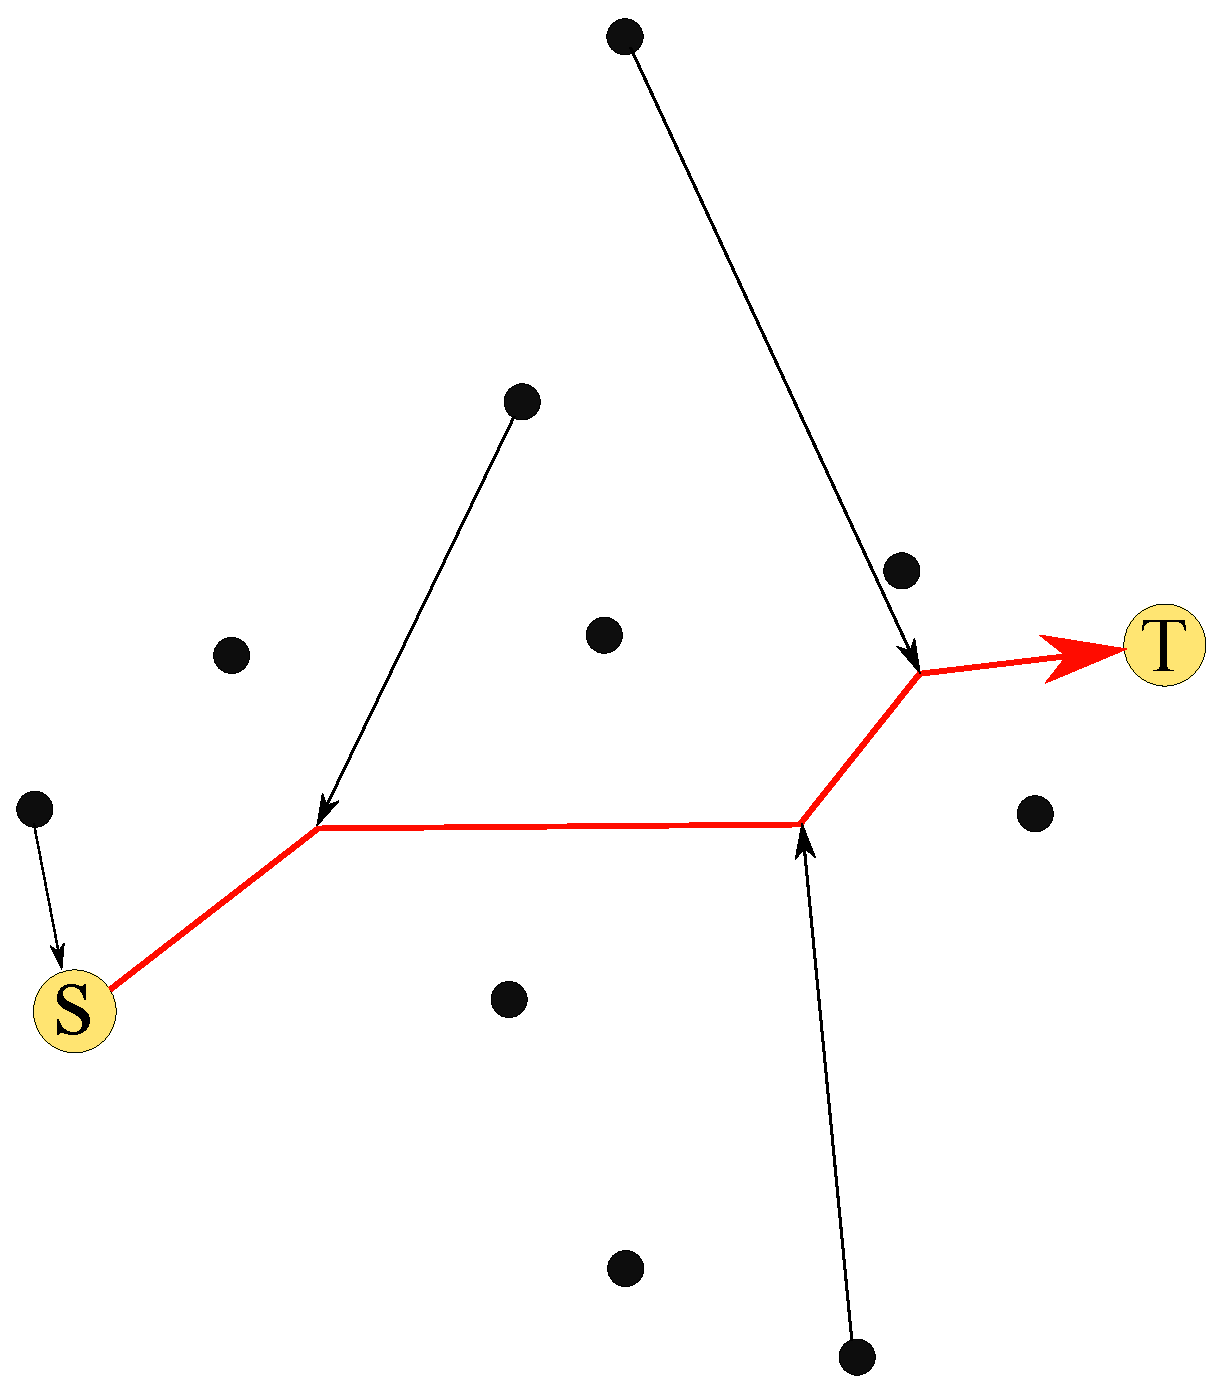
\includegraphics[width=6cm]{docs/introex.eps}
    \caption{An instance of the Package Handoff problem for a single package being transported from $S$ to $T$. 
     Agents are located at the dots marked in black. The package travels along the red path. The agents all have 
     different velocities, and in this example, assumed to have infinite battery capacity.}%
    \label{fig:introex}%
  \end{center}
\end{wrapfigure}

How do you get a package from an initial location $S$ to a destination point $T$ using a fleet of ``heterogenous'' carrier agents 
(e.g. drones, taxis). By ``heterogenous'' we mean the two agents can have different capabilities like 
different maximum speed or different fuel capacity. 


In the simplest version of the category of problems, 
we are given as input the initial locations of $n$  agents in $\mathbb{R}^2$ 
each capable of a maximum speed $u_i >0$ (where $u_i$ need not be equal to $v_j$ for $i \neq j$).
Each agent can pick up the package and move to another point to \textit{rendezvous with} and 
\textit{hand off} the 
package to another agent. This other agent then either proceeds to $T$ or decides to meet with 
and hand off the package to another agent \footnote{If it makes the package get to $T$ faster} 
and so on and so forth. 

The objective is to get the agents to cooperate to send the package from $S$ to $T$ in the 
least possible time. We call this the \textit{Package Handoff Problem}. 

To solve this problem and its various avatars 
\footnote{Say when there are multiple packages to be delivered or a bound on fuel} 
we need to 


\begin{enumerate}
\item Figure out which subset $S = \{i_1, i_2, \ldots i_k\}$ of the drones are used in the optimal schedule. 
\item Find the order in which the handoffs happend between the drones used in a schedule. 
\item Calculate the ``handoff'' points where drone $i_m$ hands over the package to drone $i_{m+1}$ 
\footnote{The last drone in the computed schedule, of course, flies directly to $T$}
\end{enumerate}

A real world instance of the basic Package Handoff problem, as described in the abstract, is when a 
ride hailing service  must co-ordinate its fleet of taxis to transport a passenger from a given location 
in the quickest possible time to the target destination on the map. In this model, 
a passenger ``hops rides'' when two taxis meet: a taxi first gets to the passenger and takes him/her to 
a point where it rendezvous with another taxi, at which point the passenger swaps taxis. This process continues 
until the passenger hops onto a taxi that goes straight to the target.  

This package handoff process is depicted in \autoref{fig:introex}. 


\section{A note on source code}
Many of the heuristics algorithms described here are implemented as literate programs \cite{Knuth:1984:LP:473.479} 
in Python 2.7.12 using the NuWeb tool \cite{briggs1992nuweb} available from \url{http://nuweb.sourceforge.net/}
alongside associated theoretical and empirical analysis. All the algorithmic code goes into the 
file \verb|pholib.py|, and any associated helper codes go into the files which are named as \verb|utils_*.py|. 
The code for these utility files has been given in the appendices. 

The \verb|pholib.py| file looks like 

%{python-mode}%
\begin{flushleft} \small\label{scrap1}\raggedright\small
\NWtarget{nuweb3}{} \verb@"src/pholib.py"@\nobreak\ {\footnotesize {3}}$\equiv$
\vspace{-1ex}
\begin{list}{}{} \item
\mbox{}\verb@@\\
\mbox{}\verb@from colorama import Fore, Style@\\
\mbox{}\verb@from matplotlib import rc@\\
\mbox{}\verb@import matplotlib as mpl@\\
\mbox{}\verb@import matplotlib.pyplot as plt@\\
\mbox{}\verb@from scipy.optimize import minimize@\\
\mbox{}\verb@from sklearn.cluster import KMeans@\\
\mbox{}\verb@import numpy as np@\\
\mbox{}\verb@import argparse, inspect, itertools, logging@\\
\mbox{}\verb@import os, time, sys@\\
\mbox{}\verb@import pprint as pp, randomcolor @\\
\mbox{}\verb@import utils_algo, utils_graphics@\\
\mbox{}\verb@@\\
\mbox{}\verb@@\hbox{$\langle\,${\itshape Algorithms}\nobreak\ {\footnotesize \NWlink{nuweb6}{6}, \ldots\ }$\,\rangle$}\verb@@\\
\mbox{}\verb@@\hbox{$\langle\,${\itshape Run Handlers}\nobreak\ {\footnotesize \NWlink{nuweb31}{31}}$\,\rangle$}\verb@@\\
\mbox{}\verb@@\hbox{$\langle\,${\itshape Plotting}\nobreak\ {\footnotesize \NWlink{nuweb38}{38}, \ldots\ }$\,\rangle$}\verb@@\\
\mbox{}\verb@@{\NWsep}
\end{list}
\vspace{-1.5ex}
\footnotesize
\begin{list}{}{\setlength{\itemsep}{-\parsep}\setlength{\itemindent}{-\leftmargin}}

\item{}
\end{list}
\vspace{4ex}
\end{flushleft}
%{/python-mode}%

The chapters are devoted to fleshing out the chunks \textlangle \verb|Algorithms|\textrangle and 
\textlangle\verb|Experiments|\textrangle.  The \newline \textlangle \verb|Run Handlers|\textrangle and 
\textlangle \verb|Plotting|\textrangle \; chunks is mainly to deal with interactive matplotlib input, 
and as such are boring and banished to the Appendix \Winkey . 

All source code files are tangled to the \verb|src| directory. The point of entry for the code are 
\verb|main*.py| which are implemented separately in the \verb|src| directory, since their contents 
can change based on what library code is being called 
for during development and testing. Since these files are very short and the mechanics clear, 
they are implemented as standalone files (i.e. not inside this document) but directly in the \verb|src| folder 
itself. To run the code in interactive mode run the code as \verb|python src/main_interactive.py| on a 
Unix / Windows terminal in the root folder of the project \footnote{This code has been tested on an 64 bit 
machine running Linux Mint 18.3 (Sylvia) running the Linux Kernel version 4.10.0-38-generic with an 
Intel(R) Core(TM) i7 CPU 960 @ 3.20GHz CPU}. 

For a short overview of previous work on this problem see Appendix. 

The \verb|README| file containing instructions for running the source code and experiments is listed in the 
appendix (also available on the Github repository)

Each of the following sections correspond to a fixed variant of the package handoff problem and describe
algorithms for that specific variant. Enough talk! Onto algorithms! 

\section{Problem: Unlimited Fuel, Different Drone Speeds}

Much of the machinery developed in solving this basic basic basic question will be generalized and extended to 
other variants of the package handoff problem. 

We repeat the problem definition and fix some notation that will be used for the remainder 
of the section 

\begin{displayquote}
  We are given as input the initial locations $P_i$ of $n$  agents in $\mathbb{R}^2$ 
each capable of a maximum speed $u_i >0$ (where $u_i$ need not be equal to $u_j$ for $i \neq j$).
Each agent can pick up the package and move to another point to \textit{rendezvous with} and 
\textit{hand off} the 
package to another agent. This other agent then either proceeds to $T$ or decides to meet with 
and hand off the package to another agent and so on. 
The objective is to get the agents to cooperate to send the package from $S$ to $T$ in the 
least possible time. 
\end{displayquote}

We represent the handoff points as follows $H_{i_1} \ldots H_{i_k}$ for $0 \leq i_0, \ldots i_k \leq n$ stand 
for points where the drones with labels $i_0, \ldots i_k$ hand the package off in that order. More precisely 
$H_{i_j}$ is the point where drone $i_{j-1}$ hands off the package to drone $i_j$ for $1 \leq j \leq k$.  

A solution to the package handoff problem is completely specified by computing the handoff points \textit{and} the 
drone ids involved in the exchange at each handoff point. 

The optimal schedule is denoted $OPT$. It is easy to see the statements of the following structural lemma always 
hold for $OPT$. 

\begin{flem}

In $OPT$
\begin{alphalist}
\item A package is always transferred to a faster drone at a handoff point. 
\item A drone handles a package at most once i.e. if a drone hands off the package, 
      it will never be involved in a handling that package again. 
\item All drones involved in the handoff start moving simultaneously at time $t=0$ 
\item No two drones wait at a rendezvous point before rendezvous happens. 
     \footnote{waiting can happen in other problem variants 
     say when there is limited fuel or only a finite set of 
     allowed rendezvous points}
\item The path of the package is a radially monotone piecewise straight polygonal curve with respect to the 
    direction ST no matter what the initial positions $P_i$ or speeds $u_i$ of the drones. 
\item $\frac{|ST|}{v_{max}}$ is a (trivial) lower bound for $OPT$, where $v_{max}$ denotes the speed of the fastest drone. 
\end{alphalist}
\end{flem}

\begin{proof}
\todo[inline]{TODO!}
\end{proof}

\newpage
\subsection{Handoff in a fixed order}
\label{ssec:fixorder}
If we know the drones involved in the handoff \textit{along with} the order of handoff 
then we can compute the handoff points --- and hence the path of the package --- exactly via 
convex optimization as outlined in Lemma \autoref{lem:fixorder}. This fact will be exploited in many 
heuristics: such methods will compute a subset of drones involved in the handoff (alongwith 
the handoff order) followed by a call to the convex program. 


\begin{figure}[H]
\centering
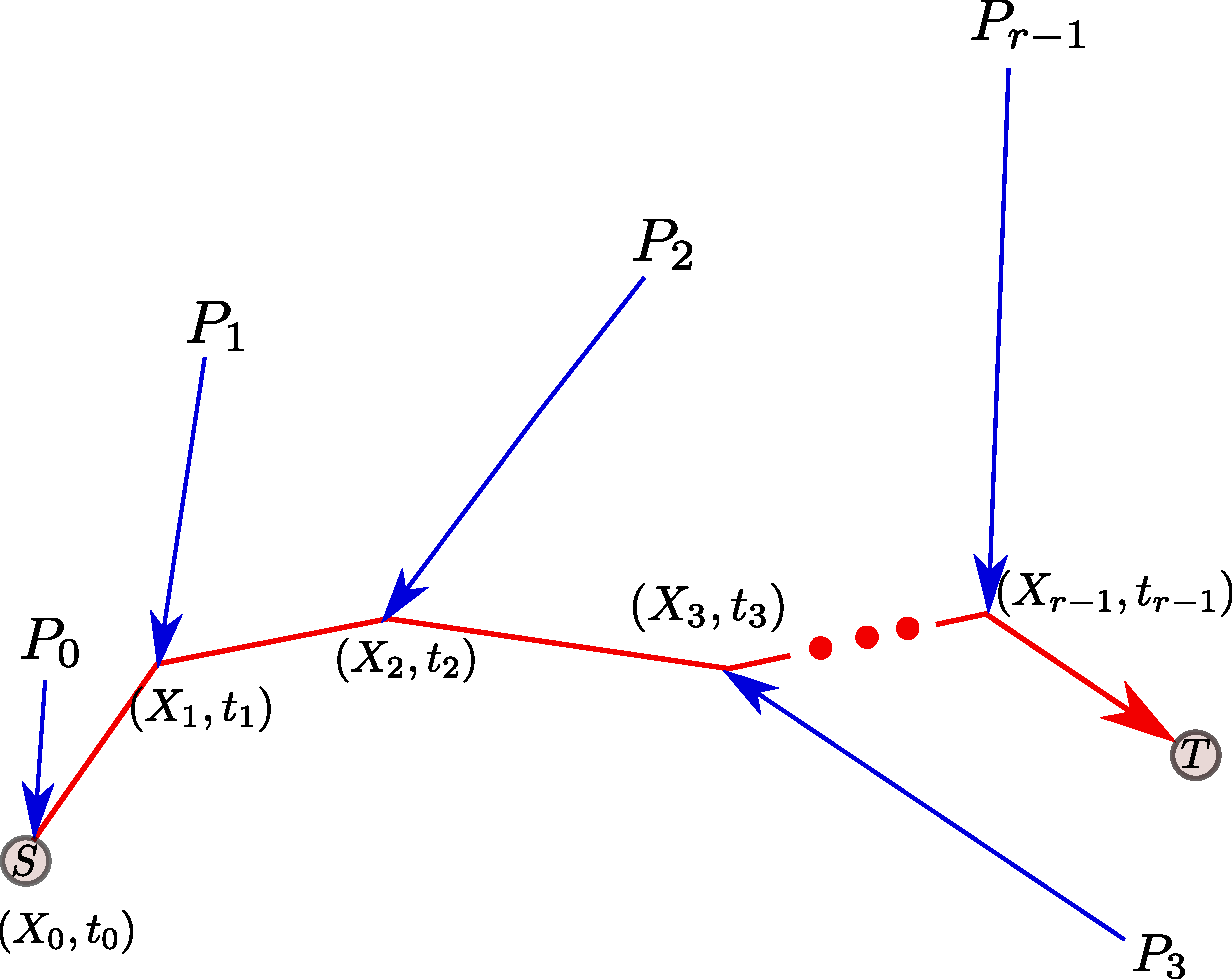
\includegraphics[width=8cm]{docs/pho-cvx.pdf}
\caption{The path of the package is shown in red. The drones invovled in the handoff are 
labelled $P_i$ in the prespecified handoff order.}
\end{figure}
\label{fig:fixorder}

\begin{flem} \label{lem:fixorder}
Given as input are drones with initial positions $P_i \in \RR^2$, with speeds $u_i>0$ 
for  $1 \leq i \leq r-1$, the intial position $S$ and final destination $T$ 
for the package. \footnote{See \autoref{fig:fixorder} for an illustration of the notation used in this lemma} 
The drones are expected to transport the package by handing of the package in the order $1,2,\ldots, r$.
Let $t_i$ denote the departure time on a global clock from the $i$'th handoff point $X_i$. 

Then the minimum time and handoff points for transporting the package and the handoff points 
can be calculated by the following convex program

\begin{equation*}
\min_{t_i, X_i} \; \; \; t_{r-1} + \frac{||T-X_{r-1}||}{u_{r-1}}
\end{equation*}

subject to the constraints

\begin{align*}
X_0 &= S\\  
t_i &\geq \frac{||P_i-X_i||}{u_i} \qquad \qquad 0 \leq i \leq r-1\\
t_i + \frac{||X_{i+1}-X_i||}{u_i} &\leq t_{i+1} \qquad \qquad \qquad \;\;\;\; 0 \leq i \leq r-2
\end{align*}

\end{flem}


The following function is just an implentation of the convex program just described. 
Here \verb|drone_info| is a list 
of tuples, where each tuple consits of the initial position and speed of the drone. The order of the 
drones is assumed to be that in which the list of drones is provided. \verb|source| and \verb|target|
are just coordinate locations of $S$ and $T$ respectively. We use the CVXPY \cite{cvxpy} library 
as a black-box convex optimization solver. 

%{python-mode}%
\begin{flushleft} \small
\begin{minipage}{\linewidth}\label{scrap2}\raggedright\small
\NWtarget{nuweb6}{} $\langle\,${\itshape Algorithms}\nobreak\ {\footnotesize {6}}$\,\rangle\equiv$
\vspace{-1ex}
\begin{list}{}{} \item
\mbox{}\verb@def algo_pho_exact_given_order_of_drones ( drone_info, source, target ):@\\
\mbox{}\verb@    import cvxpy as cp@\\
\mbox{}\verb@@\\
\mbox{}\verb@    source = np.asarray(source)@\\
\mbox{}\verb@    target = np.asarray(target)@\\
\mbox{}\verb@@\\
\mbox{}\verb@    r = len(drone_info) @\\
\mbox{}\verb@    source = np.asarray(source)@\\
\mbox{}\verb@    target = np.asarray(target)@\\
\mbox{}\verb@    @\\
\mbox{}\verb@    # Variables for rendezvous points of drone with package@\\
\mbox{}\verb@    X, t = [], []@\\
\mbox{}\verb@    for i in range(r):@\\
\mbox{}\verb@       X.append(cp.Variable(2)) # vector variable@\\
\mbox{}\verb@       t.append(cp.Variable( )) # scalar variable@\\
\mbox{}\verb@@\\
\mbox{}\verb@    # Constraints @\\
\mbox{}\verb@    constraints_S = [  X[0] == source ]@\\
\mbox{}\verb@@\\
\mbox{}\verb@    constraints_I = [] @\\
\mbox{}\verb@    for i in range(r):@\\
\mbox{}\verb@      constraints_I.append(0.0 <= t[i])@\\
\mbox{}\verb@      constraints_I.append(t[i] >= cp.norm(np.asarray(drone_info[i][0])-X[i])/drone_info[i][1])@\\
\mbox{}\verb@@\\
\mbox{}\verb@    constraints_L = []@\\
\mbox{}\verb@    for i in range(r-1):@\\
\mbox{}\verb@      constraints_L.append(t[i] + cp.norm(X[i+1] - X[i])/drone_info[i][1] <= t[i+1])@\\
\mbox{}\verb@@\\
\mbox{}\verb@    objective = cp.Minimize(t[r-1]+cp.norm(target-X[r-1])/drone_info[r-1][1])@\\
\mbox{}\verb@@\\
\mbox{}\verb@    prob = cp.Problem(objective, constraints_S + constraints_I + constraints_L)@\\
\mbox{}\verb@    print Fore.CYAN@\\
\mbox{}\verb@    prob.solve(solver=cp.SCS,verbose=True)@\\
\mbox{}\verb@    print Style.RESET_ALL@\\
\mbox{}\verb@    @\\
\mbox{}\verb@    package_trail = [ np.asarray(X[i].value) for i in range(r) ] + [ target ]@\\
\mbox{}\verb@    return package_trail@\\
\mbox{}\verb@@{\NWsep}
\end{list}
\vspace{-1.5ex}
\footnotesize
\begin{list}{}{\setlength{\itemsep}{-\parsep}\setlength{\itemindent}{-\leftmargin}}
\item \NWtxtMacroDefBy\ \NWlink{nuweb6}{6}\NWlink{nuweb7}{, 7}\NWlink{nuweb10a}{, 10a}\NWlink{nuweb12a}{, 12a}\NWlink{nuweb14a}{, 14a}\NWlink{nuweb16}{, 16}.
\item \NWtxtMacroRefIn\ \NWlink{nuweb3}{3}.

\item{}
\end{list}
\end{minipage}\vspace{4ex}
\end{flushleft}
%{/python-mode}%


We next describe a heuristic that use Continuous Dijkstra \cite{mitchell2000geometric} 
type approach in computing approximate solutions to $OPT$.

\subsection{Algorithm: One Dimensional Greedy Wavefront}
\label{ssec:odw}

In this heuristic we first constrain the package to travel along the line $\vec{ST}$, then compute the 
subset of the drones involved in the schedule, and finally pass of the list of drones involved to the convex
program given in Lemma \autoref{lem:fixorder} to calculate the rendezvous points. 


% \begin{algorithm}[H]
% \DontPrintSemicolon % Some LaTeX compilers require you to use \dontprintsemicolon instead 
% \KwIn{
% \begin{enumerate}
% \item Coordinates of initial position of source $S$ and target $T$ of the package.
% \item Coordinates of the onitial positions $P_i$ of each drone $1 \leq i \leq n$.
% \item Maximum possible speed $u_i$ of each drone $1 \leq i \leq n$. 
% \end{enumerate}

% }
% \KwOut{

% \begin{enumerate}
%  \item  \myblue{$t^*$}: The time required for the package to get from $S$ to $T$.
%  \item  \myblue{$L = (i_1, i_2, \ldots, i_k)$} : An ordered list of indices of the drones involved in the handoff. 
%  \item \myblue{$\mathcal{H} =  \{ \, S \, \} \cup \{ \, H_{i_j} \mid j\geq 2  \, \}$}:  An ordered list of handoff points.
% $H_{i_j} \in \RR^2$ is where the drone with index $i_j$ picks up the package 
%        \textit{from} drone $i_{j-1}$. 
% \end{enumerate}
% }

% \vspace{4mm}

% $t \gets 0$ \tcp*[h]{Time on the global clock} \;
% $wavelets \gets [ (i, 0) \mid 0 \leq i \leq n ]$ \tcp*[h]{Active Wavelets: indices and current radius}\;

% \vspace{2mm}
% \tcc*[h]{Find first wavelet to reach $S$ and update $wavelets$} \;

% \tcc*[h]{Start wavelet expansion from $S$} \;
% \For{$i \gets 1$ \textbf{to} $r$}{
%   \While{$n \geq c_i$} {
%     $C \gets C \cup \{c_i\}$   \;
%     $n \gets n - c_i$ 
%   }
% }
% \Return{$t^*, L, \mathcal{H}$}\;
% \caption{{\sc One dimensional greedy wavefront}}
% \label{algo:odgw}
% \end{algorithm}

\begin{figure}
    \centering
    \begin{minipage}{0.45\textwidth}
        \centering
        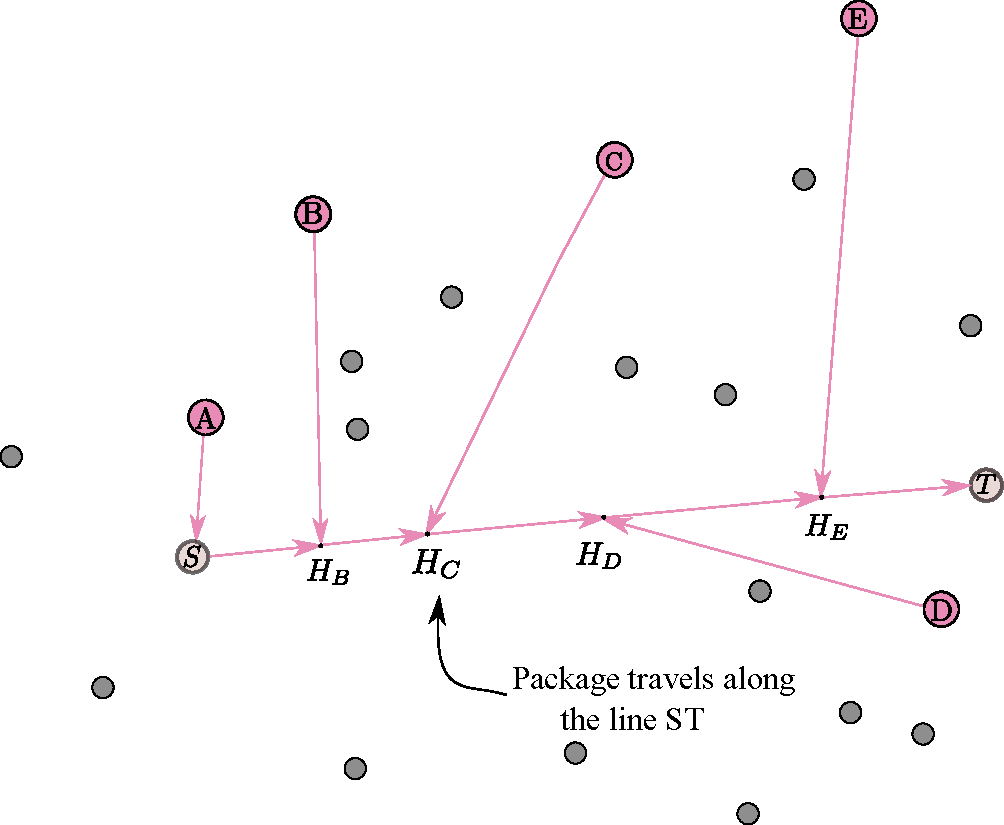
\includegraphics[width=8cm]{docs/straight-line-pho-ex.pdf}
        \caption{first figure}
     \caption{The package travels along the straight line $\vec{ST}$. The point where drone $A$ hands off the 
              package to drone $B$ depicted as $H_B$, and similarly for other drones. Drones involved in the handoff 
              are marked in pink. Those not involved are marked in gray. Two drones may have different speed.}

    \end{minipage}\hfill
    \begin{minipage}{0.45\textwidth}
        \centering
        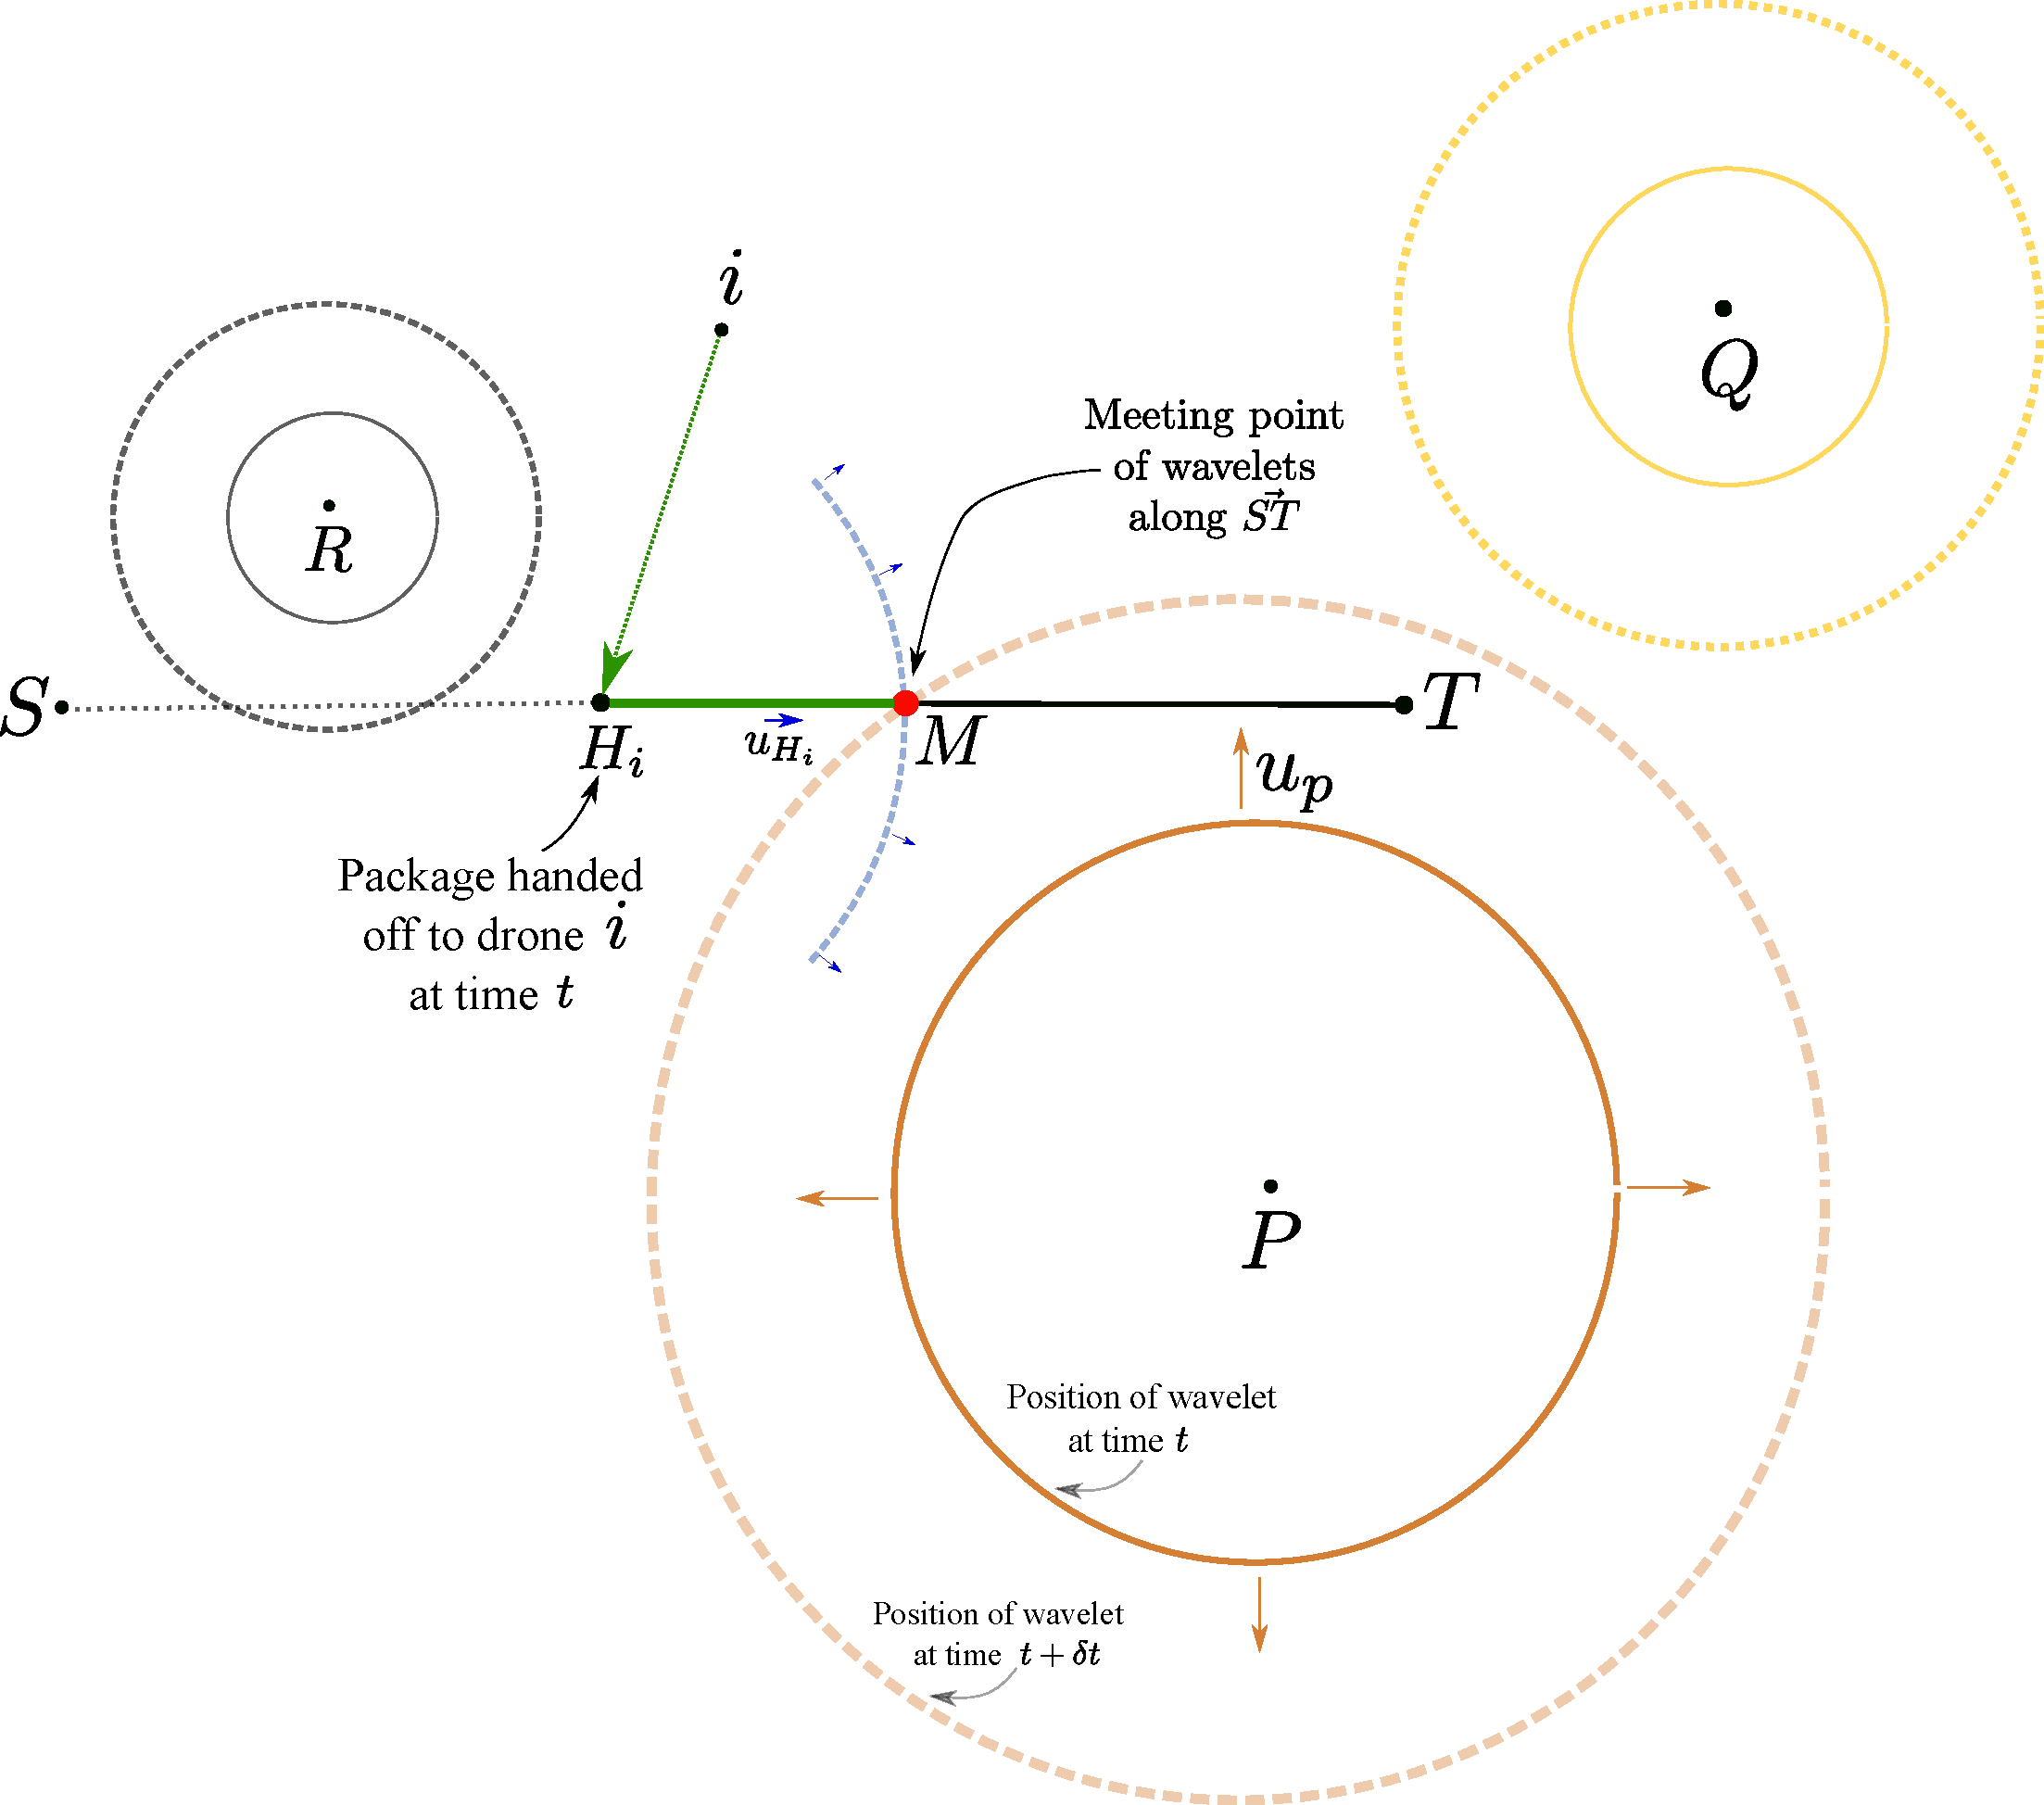
\includegraphics[width=8cm]{docs/circular_wavelets_intersect_along_st.pdf}
        \caption{second figure}
     \caption{Intersection of two expanding wavelets along $\vec{H_iT}$. The figure shows an overlay of  
              snapshots of two times; one at time $t$ (when the package has just been handed off to drone 
              $i$ at $H_i$) and another at time $t + \delta t$ (when a wavelet corresponding a drone faster 
              than drone $i$ meets it at at $M$)}
    \end{minipage}
\end{figure}
\label{fig:refalgoodw}

Here is a sketch of the implementation of \verb|algo_odw|. Use \autoref{fig:refalgoodw} as a reference while reading the
description below. 

%{python-mode}%
\begin{flushleft} \small
\begin{minipage}{\linewidth}\label{scrap3}\raggedright\small
\NWtarget{nuweb7}{} $\langle\,${\itshape Algorithms}\nobreak\ {\footnotesize {7}}$\,\rangle\equiv$
\vspace{-1ex}
\begin{list}{}{} \item
\mbox{}\verb@@\\
\mbox{}\verb@def algo_odw(drone_info, source, target, plot_tour_p = False):@\\
\mbox{}\verb@@\\
\mbox{}\verb@    from scipy.optimize import minimize@\\
\mbox{}\verb@    source     = np.asarray(source)@\\
\mbox{}\verb@    target     = np.asarray(target)@\\
\mbox{}\verb@    sthat      = (target-source)/np.linalg.norm(target-source)@\\
\mbox{}\verb@    numdrones  = len(drone_info)@\\
\mbox{}\verb@    clock_time = 0.0  # time on the global clock@\\
\mbox{}\verb@@\\
\mbox{}\verb@    @\hbox{$\langle\,${\itshape Find the drone which can get to the source the quickest}\nobreak\ {\footnotesize \NWlink{nuweb8a}{8a}}$\,\rangle$}\verb@@\\
\mbox{}\verb@    package_reached_p      = False@\\
\mbox{}\verb@@\\
\mbox{}\verb@    while not(package_reached_p):@\\
\mbox{}\verb@         @\hbox{$\langle\,${\itshape Find a faster wavelet that meets up with the package wavelet along line $\vec{ST}$ at the earliest}\nobreak\ {\footnotesize \NWlink{nuweb8b}{8b}}$\,\rangle$}\verb@        @\\
\mbox{}\verb@         @\hbox{$\langle\,${\itshape Check if package wavelet reaches target before meeting wavelet computed above. Update states accordingly}\nobreak\ {\footnotesize \NWlink{nuweb11a}{11a}}$\,\rangle$}\verb@@\\
\mbox{}\verb@@\\
\mbox{}\verb@    @\hbox{$\langle\,${\itshape Run the convex optimization solver to retrieve the exact tour \verb|package_trail_cvx| for given drone order}\nobreak\ {\footnotesize \NWlink{nuweb11c}{11c}}$\,\rangle$}\verb@      @\\
\mbox{}\verb@    @\hbox{$\langle\,${\itshape Plot tour if \verb|plot_tour_p == True|}\nobreak\ {\footnotesize \NWlink{nuweb12b}{12b}}$\,\rangle$}\verb@@\\
\mbox{}\verb@@\\
\mbox{}\verb@    return used_drones, package_trail_straight, mspan_straight, package_trail_cvx, mspan_cvx@\\
\mbox{}\verb@@{\NWsep}
\end{list}
\vspace{-1.5ex}
\footnotesize
\begin{list}{}{\setlength{\itemsep}{-\parsep}\setlength{\itemindent}{-\leftmargin}}
\item \NWtxtMacroDefBy\ \NWlink{nuweb6}{6}\NWlink{nuweb7}{, 7}\NWlink{nuweb10a}{, 10a}\NWlink{nuweb12a}{, 12a}\NWlink{nuweb14a}{, 14a}\NWlink{nuweb16}{, 16}.
\item \NWtxtMacroRefIn\ \NWlink{nuweb3}{3}.
\item \NWtxtIdentsDefed\nobreak\  \verb@algo_odw@\nobreak\ \NWlink{nuweb31}{31}.
\item{}
\end{list}
\end{minipage}\vspace{4ex}
\end{flushleft}
%{/python-mode}%
 
At the start of the algorithm, the package is stationary. We find the drone which can reach it at the earliest, 
and update the time on the global clock. It is easy to see that this drone must be involved in the optimal handoff 
schedule. 

%{python-mode}%
\begin{flushleft} \small
\begin{minipage}{\linewidth}\label{scrap4}\raggedright\small
\NWtarget{nuweb8a}{} $\langle\,${\itshape Find the drone which can get to the source the quickest}\nobreak\ {\footnotesize {8a}}$\,\rangle\equiv$
\vspace{-1ex}
\begin{list}{}{} \item
\mbox{}\verb@@\\
\mbox{}\verb@tmin = np.inf@\\
\mbox{}\verb@imin = None@\\
\mbox{}\verb@for idx in range(numdrones):@\\
\mbox{}\verb@         initdroneposn = drone_info[idx][0]@\\
\mbox{}\verb@         dronespeed    = drone_info[idx][1]@\\
\mbox{}\verb@         tmin_idx = time_of_travel(initdroneposn, source, dronespeed)@\\
\mbox{}\verb@@\\
\mbox{}\verb@         if tmin_idx < tmin:@\\
\mbox{}\verb@             tmin = tmin_idx@\\
\mbox{}\verb@             imin = idx @\\
\mbox{}\verb@@\\
\mbox{}\verb@clock_time = tmin@\\
\mbox{}\verb@@\\
\mbox{}\verb@current_package_handler_idx = imin@\\
\mbox{}\verb@current_package_position    = source@\\
\mbox{}\verb@@\\
\mbox{}\verb@drone_pool = range(numdrones)@\\
\mbox{}\verb@drone_pool.remove(imin) @\\
\mbox{}\verb@used_drones = [imin]@\\
\mbox{}\verb@package_trail_straight = [current_package_position]@\\
\mbox{}\verb@@{\NWsep}
\end{list}
\vspace{-1.5ex}
\footnotesize
\begin{list}{}{\setlength{\itemsep}{-\parsep}\setlength{\itemindent}{-\leftmargin}}
\item \NWtxtMacroRefIn\ \NWlink{nuweb7}{7}.
\item \NWtxtIdentsUsed\nobreak\  \verb@time_of_travel@\nobreak\ \NWlink{nuweb12a}{12a}.
\item{}
\end{list}
\end{minipage}\vspace{4ex}
\end{flushleft}
%{/python-mode}%

In the optimal handoff order, as we have already noted, the handoff happens from a slower to a faster robot. 
In the next chunk, we calculate the wavelet that meets the package wavelet at the earliest, subject to the 
constraint that the wavelet should be faster than the package wavelet. 


%{python-mode}%
\begin{flushleft} \small
\begin{minipage}{\linewidth}\label{scrap5}\raggedright\small
\NWtarget{nuweb8b}{} $\langle\,${\itshape Find a faster wavelet that meets up with the package wavelet along line $\vec{ST}$ at the earliest}\nobreak\ {\footnotesize {8b}}$\,\rangle\equiv$
\vspace{-1ex}
\begin{list}{}{} \item
\mbox{}\verb@   @\\
\mbox{}\verb@tI_min     = np.inf@\\
\mbox{}\verb@idx_tI_min = None@\\
\mbox{}\verb@for idx in drone_pool:@\\
\mbox{}\verb@@\\
\mbox{}\verb@      us = drone_info[current_package_handler_idx][1]@\\
\mbox{}\verb@      up = drone_info[idx][1]@\\
\mbox{}\verb@@\\
\mbox{}\verb@      if up <= us: # slower drones are useless, so skip rest of the iteration@\\
\mbox{}\verb@          continue @\\
\mbox{}\verb@      else: @\\
\mbox{}\verb@        s = current_package_position @\\
\mbox{}\verb@        p = np.asarray(drone_info[idx][0]) @\\
\mbox{}\verb@@\\
\mbox{}\verb@        tI, x = get_interception_time_and_x(s, us, p, up, target, clock_time)@\\
\mbox{}\verb@@\\
\mbox{}\verb@        if tI < tI_min:@\\
\mbox{}\verb@           tI_min     = tI@\\
\mbox{}\verb@           idx_tI_min = idx@\\
\mbox{}\verb@@{\NWsep}
\end{list}
\vspace{-1.5ex}
\footnotesize
\begin{list}{}{\setlength{\itemsep}{-\parsep}\setlength{\itemindent}{-\leftmargin}}
\item \NWtxtMacroRefIn\ \NWlink{nuweb7}{7}.
\item \NWtxtIdentsUsed\nobreak\  \verb@get_interception_time_and_x@\nobreak\ \NWlink{nuweb10a}{10a}.
\item{}
\end{list}
\end{minipage}\vspace{4ex}
\end{flushleft}
%{/python-mode}%



We now implement \verb|get_interception_time_and_x|, the time on the global clock when two wavelets meet
and position along the line $\vec{ST}$. More precisely, 
the function computes the time on the global clock at which a wavelet that started expanding from 
$P=(\alpha,\beta)$ at time 0, meets a wavelet that started expanding from $S$ at time $t_0$ along 
the half-line $\vec{ST}$. We make a change of coordinages such that $\vec{ST}$ is horizontal and 
pointing to the right, and $S=(0,0)$ as in \autoref{fig:getinterceptiontimeandx}.


\begin{figure}[H]
\centering
   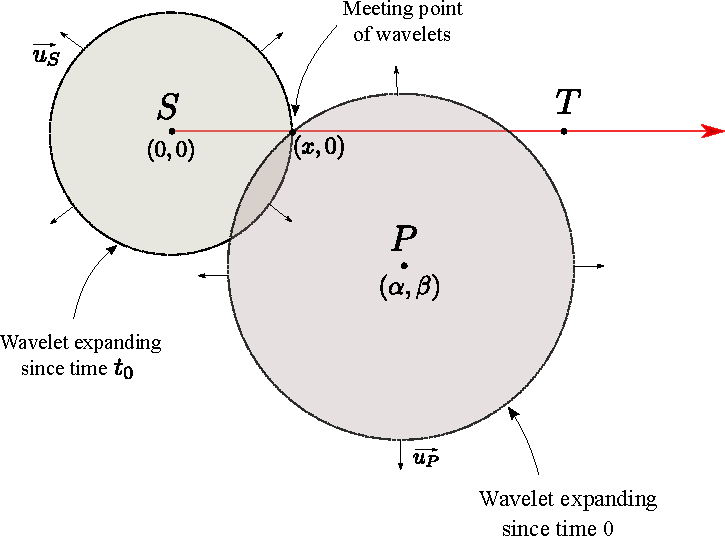
\includegraphics[width=8cm]{docs/get_interception_time_and_x.pdf}
\caption{Reference figure for the function \texttt{get\_interception\_time\_and\_x}.  
         Without loss of generality (by changing the coordinate system) we can assume 
         the line $\vec{ST}$ to be horizontal.}
\end{figure}
\label{fig:getinterceptiontimeandx}



\begin{IEEEeqnarray}{rCl}
\frac{x-0}{u_S}   &=& \frac{\sqrt{(x-\alpha)^2 + \beta^2}}{u_P} - t_0  \nonumber \\
\left(\frac{x}{u_S} + t_0 \right)^2 & = & \frac{(x-\alpha)^2 + \beta^2}{u_P^2}   \nonumber 
\end{IEEEeqnarray}


Rearranging the terms, we get a quadratic equation in $x$ that we can solve solve using standard 
non-linear solvers \footnote{Using the exact formula for solving the quadratic equation is unstable
in computer arithmetic as is well known from numerical analysis. To avoid such tricky issues, it is best
to use the standard \texttt{roots} solver for polynomials available in NumPy 
\url{https://docs.scipy.org/doc/numpy/reference/generated/numpy.roots.html}}. 

\begin{IEEEeqnarray}{rCl}
x^2 \left( \frac{1}{u_S^2} - \frac{1}{u_P^2}\right)   + x\left( \frac{2t_0}{u_S} + \frac{2\alpha}{u_P^2}\right)
+ \left(   t_0^2 - \frac{\alpha^2}{u_P^2} - \frac{\beta^2}{u_P^2} \right)    &=& 0 
\end{IEEEeqnarray}

Once we obtain $x$ getting the interception time $t_I$ (i.e. the time on the global clock 
when the two wavelets meet) as $t_I = \frac{x}{u_S} + t_0$.

%{python-mode}%
\begin{flushleft} \small
\begin{minipage}{\linewidth}\label{scrap6}\raggedright\small
\NWtarget{nuweb10a}{} $\langle\,${\itshape Algorithms}\nobreak\ {\footnotesize {10a}}$\,\rangle\equiv$
\vspace{-1ex}
\begin{list}{}{} \item
\mbox{}\verb@ @\\
\mbox{}\verb@def get_interception_time_and_x(s, us, p, up, t, t0) :@\\
\mbox{}\verb@    @\\
\mbox{}\verb@    @\hbox{$\langle\,${\itshape Change coordinates to make $s=(0,0)$ and $t$ to lie along X-axis as in \autoref{fig:getinterceptiontime}}\nobreak\ {\footnotesize \NWlink{nuweb10b}{10b}}$\,\rangle$}\verb@@\\
\mbox{}\verb@@\\
\mbox{}\verb@    # Solve quadratic equation as documented in main text@\\
\mbox{}\verb@    qroots = np.roots([ (1.0/us**2 - 1.0/up**2), @\\
\mbox{}\verb@                        2*t0/us + 2*alpha/up**2 , @\\
\mbox{}\verb@                        t0**2 - alpha**2/up**2 - beta**2/up**2])@\\
\mbox{}\verb@@\\
\mbox{}\verb@    # The quadratic should always have a root. @\\
\mbox{}\verb@    qroots = np.real(qroots) # in case the imaginary parts are really small@\\
\mbox{}\verb@    qroots.sort()            @\\
\mbox{}\verb@@\\
\mbox{}\verb@    x = None@\\
\mbox{}\verb@    for root in qroots:@\\
\mbox{}\verb@        if root > 0.0:@\\
\mbox{}\verb@           x = root@\\
\mbox{}\verb@           break@\\
\mbox{}\verb@@\\
\mbox{}\verb@    assert abs(x/us+t0 - np.sqrt((x-alpha)**2 + beta**2)/up) <= 1e-6 , \@\\
\mbox{}\verb@           "Quadratic not solved perfectly"@\\
\mbox{}\verb@@\\
\mbox{}\verb@    tI = x/us + t0@\\
\mbox{}\verb@    return tI, x@\\
\mbox{}\verb@@{\NWsep}
\end{list}
\vspace{-1.5ex}
\footnotesize
\begin{list}{}{\setlength{\itemsep}{-\parsep}\setlength{\itemindent}{-\leftmargin}}
\item \NWtxtMacroDefBy\ \NWlink{nuweb6}{6}\NWlink{nuweb7}{, 7}\NWlink{nuweb10a}{, 10a}\NWlink{nuweb12a}{, 12a}\NWlink{nuweb14a}{, 14a}\NWlink{nuweb16}{, 16}.
\item \NWtxtMacroRefIn\ \NWlink{nuweb3}{3}.
\item \NWtxtIdentsDefed\nobreak\  \verb@get_interception_time_and_x@\nobreak\ \NWlink{nuweb8b}{8b}\NWlink{nuweb16}{, 16}.
\item{}
\end{list}
\end{minipage}\vspace{4ex}
\end{flushleft}
%{/python-mode}%

Massage the input into such that $\vec{ST}$ lies along the positive X-axis as in \autoref{fig:getinterceptiontime}. 

%{python-mode}%
\begin{flushleft} \small
\begin{minipage}{\linewidth}\label{scrap7}\raggedright\small
\NWtarget{nuweb10b}{} $\langle\,${\itshape Change coordinates to make $s=(0,0)$ and $t$ to lie along X-axis as in \autoref{fig:getinterceptiontime}}\nobreak\ {\footnotesize {10b}}$\,\rangle\equiv$
\vspace{-1ex}
\begin{list}{}{} \item
\mbox{}\verb@   @\\
\mbox{}\verb@t_m = t - s # the _m subscript stands for modify@\\
\mbox{}\verb@t_m = t_m / np.linalg.norm(t_m) # normalize to unit@\\
\mbox{}\verb@@\\
\mbox{}\verb@# For rotating a vector clockwise by theta, @\\
\mbox{}\verb@# to get the vector t_m into alignment with (1,0)@\\
\mbox{}\verb@costh = t_m[0]/np.sqrt(t_m[0]**2 + t_m[1]**2)@\\
\mbox{}\verb@sinth = t_m[1]/np.sqrt(t_m[0]**2 + t_m[1]**2)@\\
\mbox{}\verb@@\\
\mbox{}\verb@rotmat = np.asarray([[costh, sinth],@\\
\mbox{}\verb@                     [-sinth, costh]])@\\
\mbox{}\verb@@\\
\mbox{}\verb@assert np.linalg.norm((rotmat.dot(t_m) - np.asarray([1,0]))) <= 1e-6,\@\\
\mbox{}\verb@       "Rotation matrix did not work properly. t_m should get rotated\@\\
\mbox{}\verb@        onto [1,0] after this transformation"@\\
\mbox{}\verb@@\\
\mbox{}\verb@p_shift  = p - s@\\
\mbox{}\verb@p_rot    = rotmat.dot(p_shift)@\\
\mbox{}\verb@[alpha, beta] = p_rot@\\
\mbox{}\verb@@{\NWsep}
\end{list}
\vspace{-1.5ex}
\footnotesize
\begin{list}{}{\setlength{\itemsep}{-\parsep}\setlength{\itemindent}{-\leftmargin}}
\item \NWtxtMacroRefIn\ \NWlink{nuweb10a}{10a}.

\item{}
\end{list}
\end{minipage}\vspace{4ex}
\end{flushleft}
%{/python-mode}%




If the package reaches the target before it meets any other wavelet along the line $\vec{ST}$, then there is no point in 
handing off the package to some other drone. Just terminate the handoff! Otherwise handoff the package and update
variables accordingly.  


%{python-mode}%
\begin{flushleft} \small
\begin{minipage}{\linewidth}\label{scrap8}\raggedright\small
\NWtarget{nuweb11a}{} $\langle\,${\itshape Check if package wavelet reaches target before meeting wavelet computed above. Update states accordingly}\nobreak\ {\footnotesize {11a}}$\,\rangle\equiv$
\vspace{-1ex}
\begin{list}{}{} \item
\mbox{}\verb@   @\\
\mbox{}\verb@time_to_target_without_handoff = np.linalg.norm((target-current_package_position))/ \@\\
\mbox{}\verb@                                 drone_info[current_package_handler_idx][1]@\\
\mbox{}\verb@@\\
\mbox{}\verb@if time_to_target_without_handoff < tI_min : @\\
\mbox{}\verb@     package_reached_p = True@\\
\mbox{}\verb@     package_trail_straight.append(target)@\\
\mbox{}\verb@@\\
\mbox{}\verb@else:@\\
\mbox{}\verb@     @\hbox{$\langle\,${\itshape Update package information (current speed, position etc.) and drone information (available and used drones)}\nobreak\ {\footnotesize \NWlink{nuweb11b}{11b}}$\,\rangle$}\verb@@\\
\mbox{}\verb@@{\NWsep}
\end{list}
\vspace{-1.5ex}
\footnotesize
\begin{list}{}{\setlength{\itemsep}{-\parsep}\setlength{\itemindent}{-\leftmargin}}
\item \NWtxtMacroRefIn\ \NWlink{nuweb7}{7}.

\item{}
\end{list}
\end{minipage}\vspace{4ex}
\end{flushleft}
%{/python-mode}%




%{python-mode}%
\begin{flushleft} \small
\begin{minipage}{\linewidth}\label{scrap9}\raggedright\small
\NWtarget{nuweb11b}{} $\langle\,${\itshape Update package information (current speed, position etc.) and drone information (available and used drones)}\nobreak\ {\footnotesize {11b}}$\,\rangle\equiv$
\vspace{-1ex}
\begin{list}{}{} \item
\mbox{}\verb@   @\\
\mbox{}\verb@package_handler_speed    = drone_info[current_package_handler_idx][1] @\\
\mbox{}\verb@current_package_position = current_package_position + \@\\
\mbox{}\verb@                            package_handler_speed * (tI_min - clock_time) *  sthat@\\
\mbox{}\verb@package_trail_straight.append(current_package_position)@\\
\mbox{}\verb@@\\
\mbox{}\verb@clock_time                  = tI_min @\\
\mbox{}\verb@current_package_handler_idx = idx_tI_min@\\
\mbox{}\verb@@\\
\mbox{}\verb@drone_pool.remove(idx_tI_min)@\\
\mbox{}\verb@used_drones.append(idx_tI_min)  @\\
\mbox{}\verb@@{\NWsep}
\end{list}
\vspace{-1.5ex}
\footnotesize
\begin{list}{}{\setlength{\itemsep}{-\parsep}\setlength{\itemindent}{-\leftmargin}}
\item \NWtxtMacroRefIn\ \NWlink{nuweb11a}{11a}.

\item{}
\end{list}
\end{minipage}\vspace{4ex}
\end{flushleft}
%{/python-mode}%


Now that we have a list of drones involved in the handoff, (along with an approximate trail for the package) 
we use the convex optimization solver to extract the exact tour for the given set of drones. We plot both tours
for a visual comparison, if \verb|plot_tour_p| is set to \verb|True|.

%{python-mode}%
\begin{flushleft} \small
\begin{minipage}{\linewidth}\label{scrap10}\raggedright\small
\NWtarget{nuweb11c}{} $\langle\,${\itshape Run the convex optimization solver to retrieve the exact tour \verb|package_trail_cvx| for given drone order}\nobreak\ {\footnotesize {11c}}$\,\rangle\equiv$
\vspace{-1ex}
\begin{list}{}{} \item
\mbox{}\verb@   @\\
\mbox{}\verb@package_trail_cvx =  algo_pho_exact_given_order_of_drones(\@\\
\mbox{}\verb@                             [drone_info[idx] for idx in used_drones],source,target)@\\
\mbox{}\verb@@\\
\mbox{}\verb@mspan_straight    = makespan(drone_info, used_drones, package_trail_straight)@\\
\mbox{}\verb@mspan_cvx         = makespan(drone_info, used_drones, package_trail_cvx)@\\
\mbox{}\verb@@{\NWsep}
\end{list}
\vspace{-1.5ex}
\footnotesize
\begin{list}{}{\setlength{\itemsep}{-\parsep}\setlength{\itemindent}{-\leftmargin}}
\item \NWtxtMacroRefIn\ \NWlink{nuweb7}{7}.

\item{}
\end{list}
\end{minipage}\vspace{4ex}
\end{flushleft}
%{/python-mode}%



The next chunk implements a function that computes the makespan of the delivery process, i.e. the time it takes
for the package to get from the source to the destination, given the points on the trajectory of the package
and the drones involved alongwith the handoff order. The variable \verb|drone_info| is list of 
tuples, where the \verb|i|\tss{th} tuple  gives the initial position and speed of the drone 
in the zeroth and first position respectively. The function \verb|time_of_travel| is simply a function
used to compute the time it takes for an agent with uniform speed to travel between a given \verb|source|
and \verb|target|. Both \verb|source| and \verb|target| are numpy arrays of size two (if not, they are converted into 
numpy arrays at the start of the function). 

%{python-mode}%
\begin{flushleft} \small
\begin{minipage}{\linewidth}\label{scrap11}\raggedright\small
\NWtarget{nuweb12a}{} $\langle\,${\itshape Algorithms}\nobreak\ {\footnotesize {12a}}$\,\rangle\equiv$
\vspace{-1ex}
\begin{list}{}{} \item
\mbox{}\verb@@\\
\mbox{}\verb@def time_of_travel(start, stop, speed):@\\
\mbox{}\verb@     start = np.asarray(start)@\\
\mbox{}\verb@     stop  = np.asarray(stop)@\\
\mbox{}\verb@     return np.linalg.norm(stop-start)/speed@\\
\mbox{}\verb@@\\
\mbox{}\verb@def extract_coordinates(points):@\\
\mbox{}\verb@@\\
\mbox{}\verb@    xs, ys = [], []@\\
\mbox{}\verb@    for pt in points:@\\
\mbox{}\verb@        xs.append(pt[0])@\\
\mbox{}\verb@        ys.append(pt[1])@\\
\mbox{}\verb@    return np.asarray(xs), np.asarray(ys)@\\
\mbox{}\verb@@\\
\mbox{}\verb@def makespan(drone_info, used_drones, package_trail):@\\
\mbox{}\verb@@\\
\mbox{}\verb@    assert len(package_trail) == len(used_drones)+1, ""@\\
\mbox{}\verb@    makespan = 0.0   @\\
\mbox{}\verb@    counter  = 0    @\\
\mbox{}\verb@    for idx in used_drones:@\\
\mbox{}\verb@         dronespeed    = drone_info[idx][1]          @\\
\mbox{}\verb@@\\
\mbox{}\verb@         makespan += time_of_travel(package_trail[counter],\@\\
\mbox{}\verb@                                    package_trail[counter+1],@\\
\mbox{}\verb@                                    dronespeed) @\\
\mbox{}\verb@         counter += 1@\\
\mbox{}\verb@    @\\
\mbox{}\verb@    return makespan@\\
\mbox{}\verb@  @\\
\mbox{}\verb@@{\NWsep}
\end{list}
\vspace{-1.5ex}
\footnotesize
\begin{list}{}{\setlength{\itemsep}{-\parsep}\setlength{\itemindent}{-\leftmargin}}
\item \NWtxtMacroDefBy\ \NWlink{nuweb6}{6}\NWlink{nuweb7}{, 7}\NWlink{nuweb10a}{, 10a}\NWlink{nuweb12a}{, 12a}\NWlink{nuweb14a}{, 14a}\NWlink{nuweb16}{, 16}.
\item \NWtxtMacroRefIn\ \NWlink{nuweb3}{3}.
\item \NWtxtIdentsDefed\nobreak\  \verb@extract_coordinates@\nobreak\ \NWlink{nuweb38}{38}\NWlink{nuweb41}{, 41}, \verb@makespan,@\nobreak\ \NWtxtIdentsNotUsed, \verb@time_of_travel@\nobreak\ \NWlink{nuweb8a}{8a}.
\item{}
\end{list}
\end{minipage}\vspace{4ex}
\end{flushleft}
%{/python-mode}%




%{python-mode}%
\begin{flushleft} \small
\begin{minipage}{\linewidth}\label{scrap12}\raggedright\small
\NWtarget{nuweb12b}{} $\langle\,${\itshape Plot tour if \verb|plot_tour_p == True|}\nobreak\ {\footnotesize {12b}}$\,\rangle\equiv$
\vspace{-1ex}
\begin{list}{}{} \item
\mbox{}\verb@   @\\
\mbox{}\verb@if plot_tour_p:@\\
\mbox{}\verb@     fig0, ax0 = plt.subplots()@\\
\mbox{}\verb@     plot_tour(fig0, ax0, "ODW: Straight Line", source, target, \@\\
\mbox{}\verb@               drone_info, used_drones, package_trail_straight)@\\
\mbox{}\verb@@\\
\mbox{}\verb@     fig1, ax1 = plt.subplots()@\\
\mbox{}\verb@     plot_tour(fig1, ax1, "ODW: Straight Line, Post Convex Optimization", source, target, \@\\
\mbox{}\verb@               drone_info, used_drones, package_trail_cvx)@\\
\mbox{}\verb@     plt.show()@\\
\mbox{}\verb@@{\NWsep}
\end{list}
\vspace{-1.5ex}
\footnotesize
\begin{list}{}{\setlength{\itemsep}{-\parsep}\setlength{\itemindent}{-\leftmargin}}
\item \NWtxtMacroRefIn\ \NWlink{nuweb7}{7}.

\item{}
\end{list}
\end{minipage}\vspace{4ex}
\end{flushleft}
%{/python-mode}%


\chapter{Multiple Package Handoff}

% \begin{figure}[H]
% \centering
% 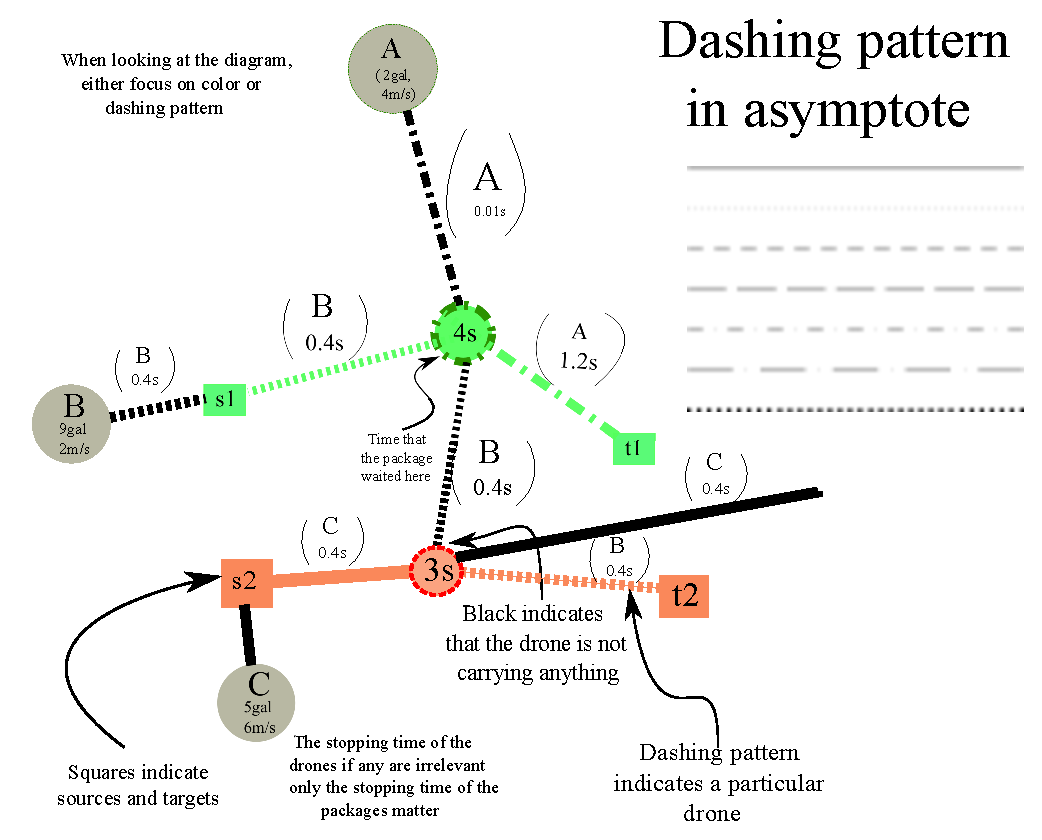
\includegraphics[width=10cm]{asy2d/example.eps}
% \end{figure}

What's more fun than delivering a single package? Delivering multiple packages! The moment, we generalize 
from a single to multiple packages the problem becomes enormously more interesting along with several 
possible generlizations to the statement of the problem. Each section is dedicated to one such generalization
along with a description of algorithms and heuristics to solve them. 

\begin{figure}[H]
\centering
\includegraphics[width=6cm]{example-grid-100x100pt}
\end{figure}
\label{fig:multiplepho-assignment}

\section{Problem: Drone Assignment To Packages}
We are given as input the initial locations $P_i$ of $n$  agents in $\mathbb{R}^2$ 
each capable of a maximum speed $u_i >0$.
Also given are $k \leq n$ source target pairs $S_j, T_j$ where $S_j$ for $j \leq k$ 
denotes the beginning position of a package that has to get to target point $T_j$.  
Each agent is allowed to be involved in the transport of at most one package. More 
than one agent is allowed to be assigned to a package. Agents  assigned to a package 
can coordinate to rendezvous and relay the package from its source to its destination 
(exactly as in the single package handoff case)

The objective is to perform an assignment of agents to the packages so that the time 
taken to deliver the last package to its target is minimized, i.e. the makespan of 
the deliveries of the packages from sources to their destinations is minimized.  
See \label{fig:multiplepho-assignment} for an example instance (alongside tours computed
for the packages and drones by the ``match and move'' algorithm to be described next.)

\subsection{Algorithm: Match-and-Move}
\label{ssec:matchmove}

The approach taken here is again based on Continuous Dijkstra. 
At the start of the algorithm, we assume each of the packages 
are constrained to travel along the the straight line segment joining 
its source and target.  We then imagine wavelets expanding at speed $u_i$ 
from each of the drone positions and perform an incremental assignment of the 
drones to the packages as the wavelet expansion proceeds. 
The assignment is done via bottleneck matching in an appropriately 
constructed bipartite graph. The matching algorithm is run everytime 
a certain ``event'' is detected. 

Once the final assignment of drones to packages has been performed, 
we run the convex optimization solver desribed in \autoref{ssec:fixorder}
to get the exact trajectory for each of the packages for the given assignment.

The rest of this section is devoted to making the above description 
more precise. First we give an outline of  \verb|algo_matchmove| that will be 
fleshed out in subsequent subsections. 

%{python-mode}%
\begin{flushleft} \small
\begin{minipage}{\linewidth}\label{scrap13}\raggedright\small
\NWtarget{nuweb14a}{} $\langle\,${\itshape Algorithms}\nobreak\ {\footnotesize {14a}}$\,\rangle\equiv$
\vspace{-1ex}
\begin{list}{}{} \item
\mbox{}\verb@import networkx as nx @\\
\mbox{}\verb@@\\
\mbox{}\verb@def algo_matchmove(drone_info, sources, targets, plot_tour_p = False):@\\
\mbox{}\verb@@\\
\mbox{}\verb@     @\hbox{$\langle\,${\itshape Sanity checks on input for \verb|algo_matchmove|}\nobreak\ {\footnotesize \NWlink{nuweb14b}{14b}}$\,\rangle$}\verb@@\\
\mbox{}\verb@     @\hbox{$\langle\,${\itshape Basic setup}\nobreak\ {\footnotesize \NWlink{nuweb17}{17}}$\,\rangle$}\verb@@\\
\mbox{}\verb@    @\\
\mbox{}\verb@     while not all(package_delivered_p):@\\
\mbox{}\verb@          @\hbox{$\langle\,${\itshape Construct bipartite graph $G$ on drone wavelets and package wavelets}\nobreak\ {\footnotesize \NWlink{nuweb19a}{19a}}$\,\rangle$}\verb@@\\
\mbox{}\verb@          @\hbox{$\langle\,${\itshape Get a bottleneck matching on $G$}\nobreak\ {\footnotesize \NWlink{nuweb20b}{20b}}$\,\rangle$}\verb@@\\
\mbox{}\verb@          @\hbox{$\langle\,${\itshape Expand drone wavelets till an event of either Type \rnum{1} or Type \rnum{2} is detected}\nobreak\ {\footnotesize \NWlink{nuweb21a}{21a}}$\,\rangle$}\verb@@\\
\mbox{}\verb@@\\
\mbox{}\verb@     @\hbox{$\langle\,${\itshape Plot movement of packages and drones if \verb|plot_tour_p == True |}\nobreak\ {\footnotesize \NWlink{nuweb23c}{23c}}$\,\rangle$}\verb@ @\\
\mbox{}\verb@     return @\\
\mbox{}\verb@     #return pass pass pass pass pass @\\
\mbox{}\verb@@{\NWsep}
\end{list}
\vspace{-1.5ex}
\footnotesize
\begin{list}{}{\setlength{\itemsep}{-\parsep}\setlength{\itemindent}{-\leftmargin}}
\item \NWtxtMacroDefBy\ \NWlink{nuweb6}{6}\NWlink{nuweb7}{, 7}\NWlink{nuweb10a}{, 10a}\NWlink{nuweb12a}{, 12a}\NWlink{nuweb14a}{, 14a}\NWlink{nuweb16}{, 16}.
\item \NWtxtMacroRefIn\ \NWlink{nuweb3}{3}.
\item \NWtxtIdentsDefed\nobreak\  \verb@algo_matchmove@\nobreak\ \NWlink{nuweb31}{31}.
\item{}
\end{list}
\end{minipage}\vspace{4ex}
\end{flushleft}
%{/python-mode}%

\subsubsection{Sanity Checks, and Basic Setup}
\label{ssec:sancheck}
To start things off, we enforce the constraint that the number of drones 
should be greater than the number of packages. Also the number of 
packages is equal to the number of sources which in turn is equal to the 
number of targets. These conditions are encoded as sanity checks 
in the code chunk below that is incorporated at the beginning of the 
function 

%{python-mode}%
\begin{flushleft} \small
\begin{minipage}{\linewidth}\label{scrap14}\raggedright\small
\NWtarget{nuweb14b}{} $\langle\,${\itshape Sanity checks on input for \verb|algo_matchmove|}\nobreak\ {\footnotesize {14b}}$\,\rangle\equiv$
\vspace{-1ex}
\begin{list}{}{} \item
\mbox{}\verb@   @\\
\mbox{}\verb@assert len(drone_info) >= len(sources),\@\\
\mbox{}\verb@   "Num drones should be >= the num source-target pairs"@\\
\mbox{}\verb@@\\
\mbox{}\verb@assert len(sources) == len(targets),\@\\
\mbox{}\verb@   "Num sources should be == Num targets"@\\
\mbox{}\verb@@{\NWsep}
\end{list}
\vspace{-1.5ex}
\footnotesize
\begin{list}{}{\setlength{\itemsep}{-\parsep}\setlength{\itemindent}{-\leftmargin}}
\item \NWtxtMacroRefIn\ \NWlink{nuweb14a}{14a}.

\item{}
\end{list}
\end{minipage}\vspace{4ex}
\end{flushleft}
%{/python-mode}%


The lists \verb|sources|, \verb|targets|, \verb|drone_initposns| and \verb|drone_speeds| 
are all \textit{constant} throughout the execution of the algorithm. They denote the list of sources, 
targets, initial position and speeds of the drones respectively. For package \verb|i|, its source and 
destination are respectively \verb|source[i]| and \verb|target[i]|. 


Then, we create some lists that keep track of various states in the 
main \texttt{while} loop of the algorithm. 

\begin{description}
\item[A. \texttt{package\_delivered\_p}] is a Boolean list
       where the \verb|i|\textsuperscript{th} element keeps track whether 
       the package with id \verb|i| has been delivered to its destination. 
       The main \verb|while| loop stops when all flags are set to \verb|True|. 
     
\item[B. \texttt{drone\_pool}] is a list of ids of drones that can be 
     considered for the bottleneck matching process for the next iteration of 
     the \verb|while| loop.  

\item[C. \texttt{drone\_wavelet\_info}] is a list of list of dictionaries. Each outer list 
     corresponds to a list of wavelets of to each drone. Every wavelet is represented
     by a dictionary, with three attributes
     
\begin{description}
  \item[1. \texttt{wavelet\_center}] The cartesian coordinates of the center $H$ of the 
          wavelet about which the wavelet expands.
  \item[2. \texttt{clock\_time}] The time on the global clock at which the wavelet started expanding around the 
         wavelet center $H$.
  \item[3. \texttt{matched\_package\_ids}] A list of the ids of the packages that were assigned to the wavelet 
     during its expansion around center $H$. Each such list is initialized as the empty list. 
\end{description}
     
     See \autoref{fig:wavelet_dict} to see a sequence of wavelets corresponding 
     to a single drone.   

\begin{figure}[H]
\centering
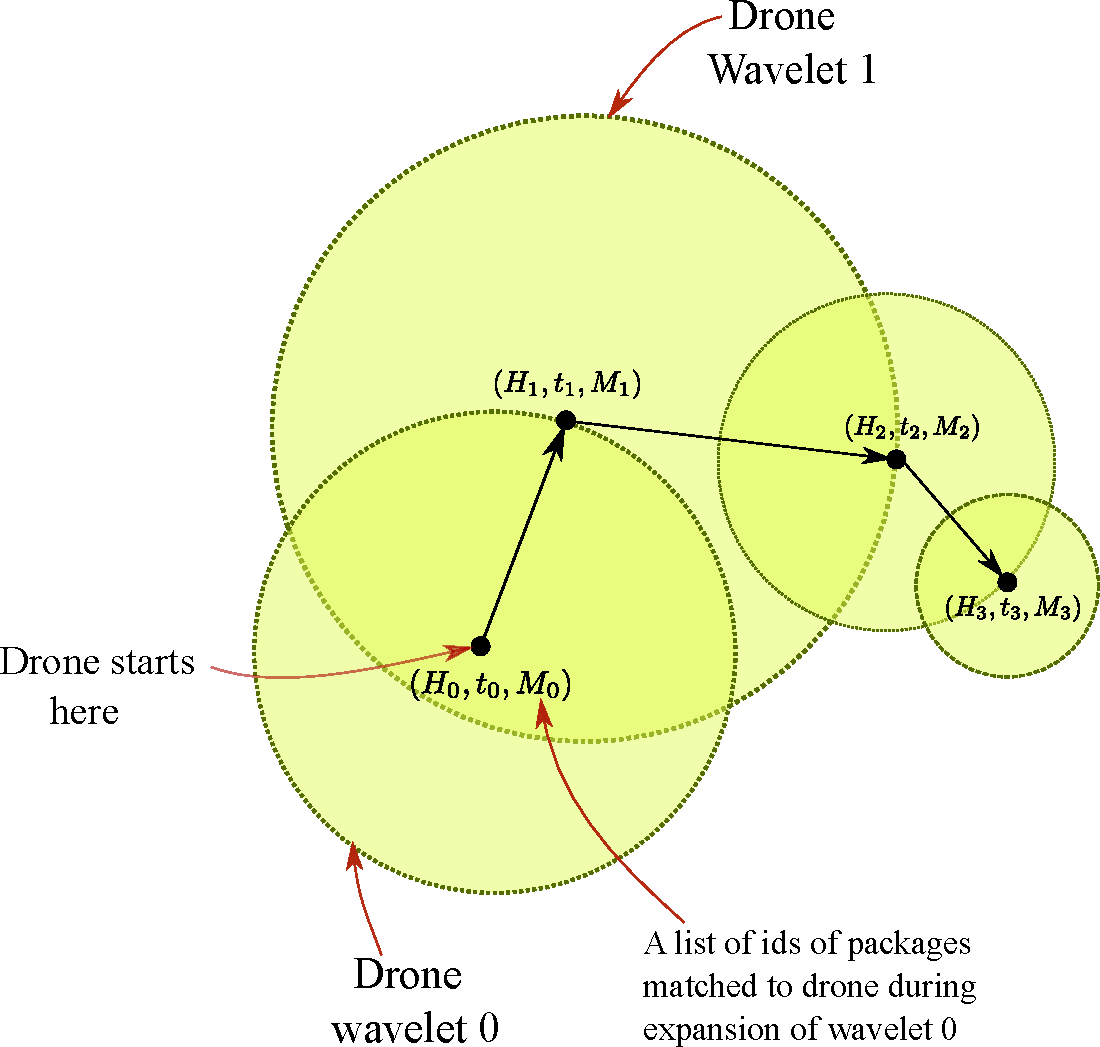
\includegraphics[width=10cm]{docs/wavelet_dict.pdf}
\caption{A sequence of wavelets corresponding to a drone which is stored as a list of dictionaries 
(each dictionary corresponding to a wavelet) 
\texttt{[\{'wavelet\_center':$H_i$, 'clock\_time':$t_i$, 'matched\_package\_ids': $M_i$\}]}.
 Each wavelet expands around $H_i$ at speed $u_i$
 starting at time $t_i$ on the global clock. Every drone has a sequence of wavelets. The $H_i$ also represent 
 handoff points where the drone either hands a package off to another drone or is handed a package by another 
 drone. Note that the usage of the letter $H$ to represent the center of
     a drone wavelet is suggestive of it also being a point where a package is handed to 
     the drone or a package is handed off to another drone.}
\end{figure}
\label{fig:wavelet_dict}


\item[D. \texttt{package\_trail\_info}]  is a list of list of dictionaries, similar to \verb|drone_wavelet_info|.  
     The \verb|i|\tss{th} element of the outer list corresponds to the trail of a package. In each trail (itself a list), we 
     record the positions of a package as well as the time on the clock $t$ at which that position was recorded. 
     We also note the id of the last drone known to have handled the package at time $t - \varepsilon$ for 
     $\varepsilon$ being an arbitrarily small positive number. 

     Two helper functions \verb|get_current_position_of_package| and \verb|get_current_speed_of_package| to extract 
     information conveniently from \verb|package_trail_info|. Again like \verb|get_last_wavelet_of_drone| the 
     result returned depends on the state of \verb|package_trail_info| at the time the function is called. 

\end{description}


We will also need a slightly generalized version of \verb|get_interception_time_and_x| that takes into
account when a wavelet started expanding in order to calculate $x$ and the time $t_I$ on the global clock
when the wavelets will meet. 


\begin{figure}[H]
\centering
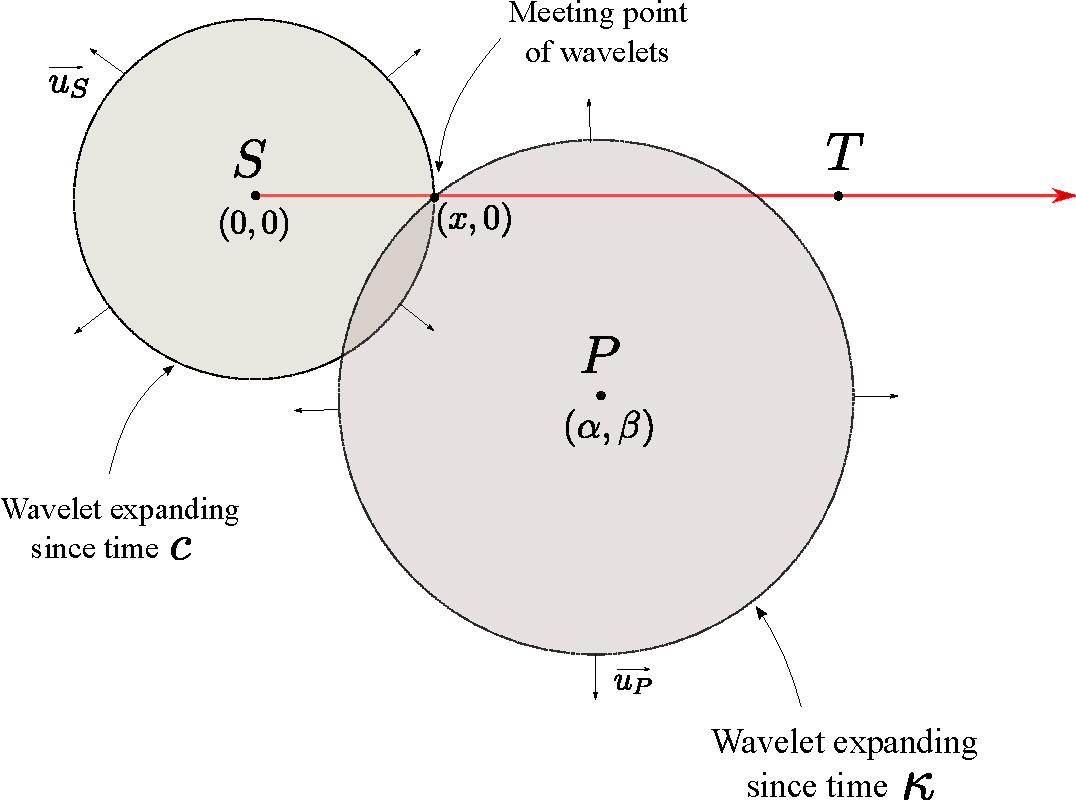
\includegraphics[width=10cm]{docs/get_interception_time_and_x_generalized.pdf}
\caption{Without loss of generality (by changing the coordinate system) we can assume 
         the line $\vec{ST}$ to be horizontal. We would like to compute the time $t_I$
         on the global clock when the two wavelets meet. The package wavelet starts expanding at 
         time $c$ which is the same as the global clock time at the moment the function is called 
         and the dronw wavelet at time $\kappa$.}
\end{figure}



%{python-mode}%
\begin{flushleft} \small
\begin{minipage}{\linewidth}\label{scrap15}\raggedright\small
\NWtarget{nuweb16}{} $\langle\,${\itshape Algorithms}\nobreak\ {\footnotesize {16}}$\,\rangle\equiv$
\vspace{-1ex}
\begin{list}{}{} \item
\mbox{}\verb@ @\\
\mbox{}\verb@def get_interception_time_and_x_generalized(s, us, p, up, t, c, k) :@\\
\mbox{}\verb@@\\
\mbox{}\verb@    assert c-k>=0 , "c, global clock time should be greater than k,\@\\
\mbox{}\verb@                    time when wavelet started expanding"@\\
\mbox{}\verb@@\\
\mbox{}\verb@    _ , x = get_interception_time_and_x(s,us,p,up,t,c-k)@\\
\mbox{}\verb@ @\\
\mbox{}\verb@    #### TODO! an assertion statement that makes sure that @\\
\mbox{}\verb@    #### c+x/us == k + |PM|/up where M is the meeting point @\\
\mbox{}\verb@    #### of the wavelets@\\
\mbox{}\verb@@\\
\mbox{}\verb@    return c+x/us, x@\\
\mbox{}\verb@@{\NWsep}
\end{list}
\vspace{-1.5ex}
\footnotesize
\begin{list}{}{\setlength{\itemsep}{-\parsep}\setlength{\itemindent}{-\leftmargin}}
\item \NWtxtMacroDefBy\ \NWlink{nuweb6}{6}\NWlink{nuweb7}{, 7}\NWlink{nuweb10a}{, 10a}\NWlink{nuweb12a}{, 12a}\NWlink{nuweb14a}{, 14a}\NWlink{nuweb16}{, 16}.
\item \NWtxtMacroRefIn\ \NWlink{nuweb3}{3}.
\item \NWtxtIdentsUsed\nobreak\  \verb@get_interception_time_and_x@\nobreak\ \NWlink{nuweb10a}{10a}.
\item{}
\end{list}
\end{minipage}\vspace{4ex}
\end{flushleft}
%{/python-mode}%



%{python-mode}%
\begin{flushleft} \small
\begin{minipage}{\linewidth}\label{scrap16}\raggedright\small
\NWtarget{nuweb17}{} $\langle\,${\itshape Basic setup}\nobreak\ {\footnotesize {17}}$\,\rangle\equiv$
\vspace{-1ex}
\begin{list}{}{} \item
\mbox{}\verb@ @\\
\mbox{}\verb@sources             = [np.asarray(source) for source in sources] @\\
\mbox{}\verb@targets             = [np.asarray(target) for target in targets] @\\
\mbox{}\verb@@\\
\mbox{}\verb@drone_initposns     = [ np.asarray(initposn) for (initposn, _) in drone_info ]@\\
\mbox{}\verb@drone_speeds        = [ speed                for (_,    speed) in drone_info ]@\\
\mbox{}\verb@@\\
\mbox{}\verb@numpackages         = len(sources) @\\
\mbox{}\verb@numdrones           = len(drone_info)@\\
\mbox{}\verb@@\\
\mbox{}\verb@# State variables that change during the main loop@\\
\mbox{}\verb@package_delivered_p = [ False for _ in range(numpackages) ] @\\
\mbox{}\verb@drone_locked_p      = [ False for _ in range(numdrones)   ]@\\
\mbox{}\verb@drone_pool          = range(numdrones)@\\
\mbox{}\verb@remaining_packages  = range(numpackages)@\\
\mbox{}\verb@global_clock_time   = 0.0@\\
\mbox{}\verb@drone_wavelets_info = [ [{'wavelet_center'        : posn,@\\
\mbox{}\verb@                          'clock_time'            : 0.0,@\\
\mbox{}\verb@                          'matched_package_ids'   : []}] @\\
\mbox{}\verb@                        for posn in drone_initposns ]@\\
\mbox{}\verb@package_trail_info  = [ [{'current_position'   : source, @\\
\mbox{}\verb@                          'clock_time'         : 0.0,@\\
\mbox{}\verb@                          'current_handler_id' : None }] @\\
\mbox{}\verb@                        for source in sources ]@\\
\mbox{}\verb@@\\
\mbox{}\verb@# Useful functions for extracting information from state variables above@\\
\mbox{}\verb@def get_last_wavelet_of_drone(i):@\\
\mbox{}\verb@         return drone_wavelets_info[i][-1]@\\
\mbox{}\verb@@\\
\mbox{}\verb@def get_current_position_of_package(i):@\\
\mbox{}\verb@         return package_trail_info[i][-1]['current_position']@\\
\mbox{}\verb@    @\\
\mbox{}\verb@def get_current_speed_of_package(i):@\\
\mbox{}\verb@         current_handler_id = package_trail_info[i][-1]['current_handler_id']@\\
\mbox{}\verb@@\\
\mbox{}\verb@         if current_handler_id is None:@\\
\mbox{}\verb@              return 0.0@\\
\mbox{}\verb@         else:@\\
\mbox{}\verb@              return drone_speeds[current_handler_id]@\\
\mbox{}\verb@@\\
\mbox{}\verb@def get_current_handler_of_package(i):@\\
\mbox{}\verb@         return package_trail_info[i][-1]['current_handler_id']@\\
\mbox{}\verb@@\\
\mbox{}\verb@def dronelabel(idx):@\\
\mbox{}\verb@    return 'drone_' + str(idx)@\\
\mbox{}\verb@@\\
\mbox{}\verb@def packagelabel(idx):@\\
\mbox{}\verb@    return 'package_' + str(idx)@\\
\mbox{}\verb@@{\NWsep}
\end{list}
\vspace{-1.5ex}
\footnotesize
\begin{list}{}{\setlength{\itemsep}{-\parsep}\setlength{\itemindent}{-\leftmargin}}
\item \NWtxtMacroRefIn\ \NWlink{nuweb14a}{14a}.
\item \NWtxtIdentsDefed\nobreak\  \verb@dronelabel,@\nobreak\ \NWtxtIdentsNotUsed, \verb@get_current_position_of_package,@\nobreak\ \NWtxtIdentsNotUsed, \verb@get_current_speed_of_package,@\nobreak\ \NWtxtIdentsNotUsed, \verb@get_last_wavelet_of_drone,@\nobreak\ \NWtxtIdentsNotUsed, \verb@packagelabel@\nobreak\ \NWlink{nuweb19a}{19a}.
\item{}
\end{list}
\end{minipage}\vspace{4ex}
\end{flushleft}
%{/python-mode}%

 The \verb|get_wavelet_of_drone| function defined at the end of the above chunk is a convenience function 
 for returning the center of the last wavelet and the associated clock time recorded at that center
 for an arbitrary drone.  \textbf{Note:} The result of calling this function depends on the time at which it 
 is called because \verb|drone_wavelet_info| list is mutated during the main while loop.

\subsubsection{Main Loop}
\label{ssec:mainloopmatchmove}

% Each iteration corresponds to processing exactly one event. There are 
% exactly two types of (mutually exclusive) events in this algorithm. 

% \begin{description}
% \item[Type \rnum{1}:] A package gets delivered to its assigned destination. 
% \item[Type \rnum{2}:] A wavelet corresponding to a drone (not handling a package) meets up with 
%    a drone currently handling a package. 
% \end{description}

% In both event types, a drone gets taken out of the drone pool:  for 
% the Type \rnum{1} event the 
% drone that just delivered the package to the destination; for the Type 
% \rnum{2} event the drone that just handed off the package. 

It is critical that the zero testing for upkg has 
been done for \verb|time_target_to_solo| to be computed safely 
without worrying about \verb|ZeroDivisionError|.

Note that the graph bipartite $G$ is encoded as a matrix of weights as shown in the 
figure \autoref{fig:bipart}

\begin{figure}[H]
\centering
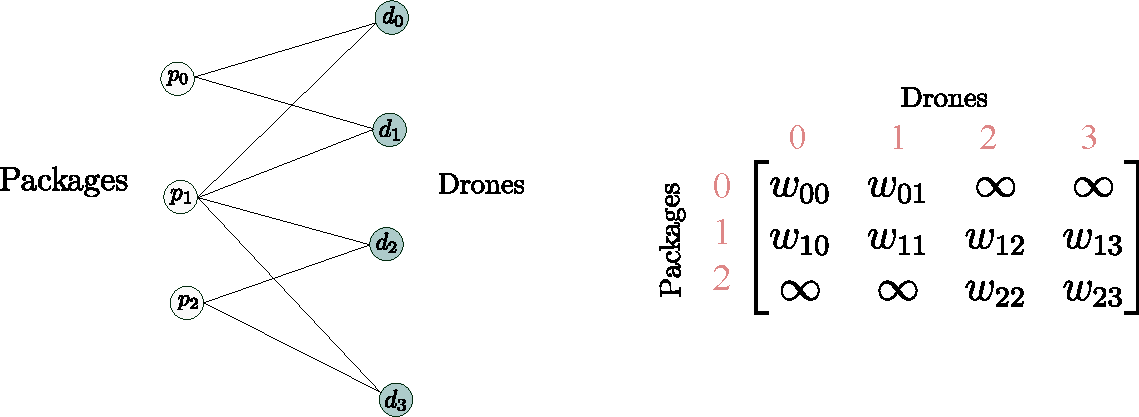
\includegraphics[width=17cm]{docs/bipartgraph_demo.pdf}
\caption{A bipartite graph $G$ constructed between the drones 
and packages, along witht the asosciated weight matrix. Edges between
drones and packages not in the graph are represented by infinite edge 
weights. A minimum weight bipartite matching algorithm from SciPy (\url{http://bit.ly/2MAWHPn}) will 
be used as a replacement for bottleneck matching (SciPy / NetworkX do not 
have such a solver) The matrix shown in the right half of the above figure is 
built inside the code, one column at a time. }
\end{figure}
\label{fig:bipart}

%{python-mode}%
\begin{flushleft} \small
\begin{minipage}{\linewidth}\label{scrap17}\raggedright\small
\NWtarget{nuweb19a}{} $\langle\,${\itshape Construct bipartite graph $G$ on drone wavelets and package wavelets}\nobreak\ {\footnotesize {19a}}$\,\rangle\equiv$
\vspace{-1ex}
\begin{list}{}{} \item
\mbox{}\verb@  @\\
\mbox{}\verb@infty       = np.inf @\\
\mbox{}\verb@G_mat       = np.full((len(remaining_packages),len(drone_pool)), infty)@\\
\mbox{}\verb@lbend_edges = []@\\
\mbox{}\verb@zerotol = 1e-7@\\
\mbox{}\verb@@\\
\mbox{}\verb@for didx in drone_pool:@\\
\mbox{}\verb@    dlabel = dronelabel(didx)@\\
\mbox{}\verb@@\\
\mbox{}\verb@    for pidx in remaining_packages: @\\
\mbox{}\verb@        current_handler_of_package = get_current_handler_of_package(pidx)@\\
\mbox{}\verb@@\\
\mbox{}\verb@        if  ((current_handler_of_package is None)  or current_handler_of_package != didx) and not(drone_locked_p[didx]):@\\
\mbox{}\verb@                plabel, target = packagelabel(pidx)                   , targets[pidx]@\\
\mbox{}\verb@                pkg   , upkg   = get_current_position_of_package(pidx), get_current_speed_of_package(pidx)@\\
\mbox{}\verb@                wav            = get_last_wavelet_of_drone(didx)@\\
\mbox{}\verb@                dro   , udro   = wav['wavelet_center']                , drone_speeds[didx]@\\
\mbox{}\verb@@\\
\mbox{}\verb@                if upkg < zerotol :@\\
\mbox{}\verb@                      @\hbox{$\langle\,${\itshape Insert edge incident to stationary package and a drone}\nobreak\ {\footnotesize \NWlink{nuweb19b}{19b}}$\,\rangle$}\verb@                      @\\
\mbox{}\verb@                elif udro > upkg and abs(upkg-udro) > zerotol:@\\
\mbox{}\verb@                      @\hbox{$\langle\,${\itshape Insert edge incident to a moving package and a faster unlocked drone}\nobreak\ {\footnotesize \NWlink{nuweb20a}{20a}}$\,\rangle$}\verb@@\\
\mbox{}\verb@@\\
\mbox{}\verb@        elif current_handler_of_package == didx and drone_locked_p[didx]:@\\
\mbox{}\verb@               assert abs(udro-upkg) < zerotol , "udro should be equal to upkg"@\\
\mbox{}\verb@               G_mat[pidx, didx] = np.linalg.norm((target-pkg))/udro@\\
\mbox{}\verb@    @\\
\mbox{}\verb@        elif  ((current_handler_of_package is None)  or current_handler_of_package != didx)     and drone_locked_p[didx]:@\\
\mbox{}\verb@               pass # drone locked, so it cant help, keep the edge weight infinite@\\
\mbox{}\verb@        else : @\\
\mbox{}\verb@               # The outer not negates the inner condition which is true if this branch is executed@\\
\mbox{}\verb@               assert not(current_handler_of_package == didx and not(drone_locked_p[didx])) ,\@\\
\mbox{}\verb@            "This else branch should not be executed. This means didx is handling a package and is NOT locked"@\\
\mbox{}\verb@@{\NWsep}
\end{list}
\vspace{-1.5ex}
\footnotesize
\begin{list}{}{\setlength{\itemsep}{-\parsep}\setlength{\itemindent}{-\leftmargin}}
\item \NWtxtMacroRefIn\ \NWlink{nuweb14a}{14a}.
\item \NWtxtIdentsUsed\nobreak\  \verb@packagelabel@\nobreak\ \NWlink{nuweb17}{17}.
\item{}
\end{list}
\end{minipage}\vspace{4ex}
\end{flushleft}
%{/python-mode}%


%{python-mode}%
\begin{flushleft} \small
\begin{minipage}{\linewidth}\label{scrap18}\raggedright\small
\NWtarget{nuweb19b}{} $\langle\,${\itshape Insert edge incident to stationary package and a drone}\nobreak\ {\footnotesize {19b}}$\,\rangle\equiv$
\vspace{-1ex}
\begin{list}{}{} \item
\mbox{}\verb@   @\\
\mbox{}\verb@G_mat[pidx, didx] = np.linalg.norm(pkg-dro)/udro +\@\\
\mbox{}\verb@                    np.linalg.norm(target-pkg)/udro@\\
\mbox{}\verb@lbend_edges.append({'edge_pair': (pidx,didx), @\\
\mbox{}\verb@                    'y'        : np.linalg.norm(pkg-dro)/udro }) @\\
\mbox{}\verb@@{\NWsep}
\end{list}
\vspace{-1.5ex}
\footnotesize
\begin{list}{}{\setlength{\itemsep}{-\parsep}\setlength{\itemindent}{-\leftmargin}}
\item \NWtxtMacroRefIn\ \NWlink{nuweb19a}{19a}.

\item{}
\end{list}
\end{minipage}\vspace{4ex}
\end{flushleft}
%{/python-mode}%





%{python-mode}%
\begin{flushleft} \small
\begin{minipage}{\linewidth}\label{scrap19}\raggedright\small
\NWtarget{nuweb20a}{} $\langle\,${\itshape Insert edge incident to a moving package and a faster unlocked drone}\nobreak\ {\footnotesize {20a}}$\,\rangle\equiv$
\vspace{-1ex}
\begin{list}{}{} \item
\mbox{}\verb@   @\\
\mbox{}\verb@time_to_target_solo = np.linalg.norm(target-pkg)/upkg@\\
\mbox{}\verb@tI, x  = get_interception_time_and_x_generalized(pkg, upkg, dro, udro, target, @\\
\mbox{}\verb@                                                global_clock_time, wav['clock_time'])@\\
\mbox{}\verb@if x is not None: @\\
\mbox{}\verb@   assert tI is not None, "tI and x should be None or not None simultaneously"@\\
\mbox{}\verb@   if tI < global_clock_time + time_to_target_solo:@\\
\mbox{}\verb@@\\
\mbox{}\verb@     pthat             = (target-pkg)/np.linalg.norm(target-pkg)@\\
\mbox{}\verb@     interception_pt   = pkg + x * pthat@\\
\mbox{}\verb@     G_mat[pidx, didx] = tI + np.linalg.norm((target-interception_pt))/udro@\\
\mbox{}\verb@     lbend_edges.append({'edge_pair': (pidx,didx), @\\
\mbox{}\verb@                         'y'       : np.linalg.norm(interception_pt-dro)/udro }) @\\
\mbox{}\verb@@{\NWsep}
\end{list}
\vspace{-1.5ex}
\footnotesize
\begin{list}{}{\setlength{\itemsep}{-\parsep}\setlength{\itemindent}{-\leftmargin}}
\item \NWtxtMacroRefIn\ \NWlink{nuweb19a}{19a}.

\item{}
\end{list}
\end{minipage}\vspace{4ex}
\end{flushleft}
%{/python-mode}%





Since NetworkX does not have a native bottleneck matching solver, we use a minimum-weight matching solver
already present in SciPy documented at \url{http://bit.ly/2MAWHPn}. 

%{python-mode}%
\begin{flushleft} \small
\begin{minipage}{\linewidth}\label{scrap20}\raggedright\small
\NWtarget{nuweb20b}{} $\langle\,${\itshape Get a bottleneck matching on $G$}\nobreak\ {\footnotesize {20b}}$\,\rangle\equiv$
\vspace{-1ex}
\begin{list}{}{} \item
\mbox{}\verb@@\\
\mbox{}\verb@from scipy.optimize import linear_sum_assignment@\\
\mbox{}\verb@pkg_ind, dro_ind = linear_sum_assignment(G_mat)@\\
\mbox{}\verb@assert len(pkg_ind) == len(dro_ind), "Lengths of the index arrays should be the same"@\\
\mbox{}\verb@@{\NWsep}
\end{list}
\vspace{-1.5ex}
\footnotesize
\begin{list}{}{\setlength{\itemsep}{-\parsep}\setlength{\itemindent}{-\leftmargin}}
\item \NWtxtMacroRefIn\ \NWlink{nuweb14a}{14a}.

\item{}
\end{list}
\end{minipage}\vspace{4ex}
\end{flushleft}
%{/python-mode}%

There are exactly two types of (mutually exclusive) events in this algorithm. 

\begin{description}
\item[Type \rnum{1}:] A package wavelet reaches its target. 
\item[Type \rnum{2}:] A wavelet corresponding to a drone (not handling a package) 
                      meets up with a package wavelet.
\end{description}

To detect these, we keep track of a so-called list of ``$L$ bend'' edges as shown in the figure below 
(see the variable \verb|lbend_edges| in the previous chunk that keeps track of this quantity).  

\begin{figure}[H]
\centering
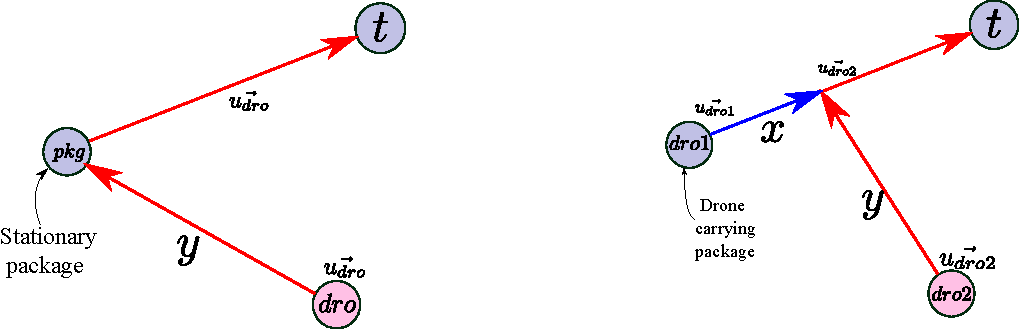
\includegraphics[width=18cm]{docs/lbend.pdf}
\caption{If a package drone pair is represented in the graph matrix as a finite weight edge, we first 
check if it is an $L$-bend edge that corresponds to one of the two situations above. A drone catches
up with another drone carrying the package (right) or a drone picks up a stationary package and moves
towards the target (left)}
\end{figure}


%{python-mode}%
\begin{flushleft} \small
\begin{minipage}{\linewidth}\label{scrap21}\raggedright\small
\NWtarget{nuweb21a}{} $\langle\,${\itshape Expand drone wavelets till an event of either Type \rnum{1} or Type \rnum{2} is detected}\nobreak\ {\footnotesize {21a}}$\,\rangle\equiv$
\vspace{-1ex}
\begin{list}{}{} \item
\mbox{}\verb@   @\\
\mbox{}\verb@@\hbox{$\langle\,${\itshape Classify edges according to whether they are straight edges or lbend edges}\nobreak\ {\footnotesize \NWlink{nuweb21b}{21b}}$\,\rangle$}\verb@@\\
\mbox{}\verb@@\hbox{$\langle\,${\itshape Get lowest weight edge (with its weight denoted emin) in the computed matching}\nobreak\ {\footnotesize \NWlink{nuweb21c}{21c}}$\,\rangle$}\verb@@\\
\mbox{}\verb@@\hbox{$\langle\,${\itshape Check if there is an lbend edge in the matching which has a $y\leq ewmin$. If so, find the one with the one with the lowest such $y$}\nobreak\ {\footnotesize \NWlink{nuweb22a}{22a}}$\,\rangle$}\verb@@\\
\mbox{}\verb@@\\
\mbox{}\verb@if ymin > ewmin:  # TYPE I EVENT (package reaches target)@\\
\mbox{}\verb@@\\
\mbox{}\verb@    assert (pmin,dmin) not in [ d['edge_pair']  for d in lbend_edges_of_matching ], " "@\\
\mbox{}\verb@    time_till_event    = ewmin@\\
\mbox{}\verb@    global_clock_time += time_till_event@\\
\mbox{}\verb@@\\
\mbox{}\verb@    @\hbox{$\langle\,${\itshape Process lbend edges in the matching for type \rnum{1} event}\nobreak\ {\footnotesize \NWlink{nuweb22b}{22b}}$\,\rangle$}\verb@@\\
\mbox{}\verb@    @\hbox{$\langle\,${\itshape Process straight edges in the matching for type \rnum{1} event}\nobreak\ {\footnotesize \NWlink{nuweb22c}{22c}}$\,\rangle$}\verb@@\\
\mbox{}\verb@    @\\
\mbox{}\verb@else:# TYPE II EVENT (a wavelet corresponding to a drone not handling @\\
\mbox{}\verb@     # a package reaches a package that might be stationary or being @\\
\mbox{}\verb@     # moved by another drone.)@\\
\mbox{}\verb@@\\
\mbox{}\verb@    assert (plmin is not None and dlmin is not None), ""@\\
\mbox{}\verb@    time_till_event    = ymin@\\
\mbox{}\verb@    global_clock_time += time_till_event@\\
\mbox{}\verb@@\\
\mbox{}\verb@    @\hbox{$\langle\,${\itshape Process lbend edges in the matching for type \rnum{2} event}\nobreak\ {\footnotesize \NWlink{nuweb23a}{23a}}$\,\rangle$}\verb@@\\
\mbox{}\verb@    @\hbox{$\langle\,${\itshape Process straight edges in the matching for type \rnum{2} event}\nobreak\ {\footnotesize \NWlink{nuweb23b}{23b}}$\,\rangle$}\verb@@\\
\mbox{}\verb@@\\
\mbox{}\verb@@{\NWsep}
\end{list}
\vspace{-1.5ex}
\footnotesize
\begin{list}{}{\setlength{\itemsep}{-\parsep}\setlength{\itemindent}{-\leftmargin}}
\item \NWtxtMacroRefIn\ \NWlink{nuweb14a}{14a}.

\item{}
\end{list}
\end{minipage}\vspace{4ex}
\end{flushleft}
%{/python-mode}%


%{python-mode}%
\begin{flushleft} \small
\begin{minipage}{\linewidth}\label{scrap22}\raggedright\small
\NWtarget{nuweb21b}{} $\langle\,${\itshape Classify edges according to whether they are straight edges or lbend edges}\nobreak\ {\footnotesize {21b}}$\,\rangle\equiv$
\vspace{-1ex}
\begin{list}{}{} \item
\mbox{}\verb@ @\\
\mbox{}\verb@lbend_edges_of_matching    = [ d for d in lbend_edges if d['edge_pair'] in zip(pkg_ind, dro_ind) ] @\\
\mbox{}\verb@straight_edges_of_matching = list(  set(zip(pkg_ind,dro_ind)).difference(\@\\
\mbox{}\verb@                                                set([d['edge_pair'] for d in lbend_edges_of_matching]))   )@\\
\mbox{}\verb@@{\NWsep}
\end{list}
\vspace{-1.5ex}
\footnotesize
\begin{list}{}{\setlength{\itemsep}{-\parsep}\setlength{\itemindent}{-\leftmargin}}
\item \NWtxtMacroRefIn\ \NWlink{nuweb21a}{21a}.

\item{}
\end{list}
\end{minipage}\vspace{4ex}
\end{flushleft}
%{/python-mode}%


%{python-mode}%
\begin{flushleft} \small
\begin{minipage}{\linewidth}\label{scrap23}\raggedright\small
\NWtarget{nuweb21c}{} $\langle\,${\itshape Get lowest weight edge (with its weight denoted emin) in the computed matching}\nobreak\ {\footnotesize {21c}}$\,\rangle\equiv$
\vspace{-1ex}
\begin{list}{}{} \item
\mbox{}\verb@@\\
\mbox{}\verb@imin  = 0@\\
\mbox{}\verb@ewmin = np.inf@\\
\mbox{}\verb@for pidx, didx, i in zip(pkg_ind, dro_ind, range(len(pkg_ind))):@\\
\mbox{}\verb@    edgewt = G_mat[pidx, didx]@\\
\mbox{}\verb@    if edgewt < ewmin :@\\
\mbox{}\verb@          imin, ewmin  = i, edgewt@\\
\mbox{}\verb@          @\\
\mbox{}\verb@pmin, dmin = pkg_ind[imin], dro_ind[imin]@\\
\mbox{}\verb@@{\NWsep}
\end{list}
\vspace{-1.5ex}
\footnotesize
\begin{list}{}{\setlength{\itemsep}{-\parsep}\setlength{\itemindent}{-\leftmargin}}
\item \NWtxtMacroRefIn\ \NWlink{nuweb21a}{21a}.

\item{}
\end{list}
\end{minipage}\vspace{4ex}
\end{flushleft}
%{/python-mode}%


%{python-mode}%
\begin{flushleft} \small
\begin{minipage}{\linewidth}\label{scrap24}\raggedright\small
\NWtarget{nuweb22a}{} $\langle\,${\itshape Check if there is an lbend edge in the matching which has a $y\leq ewmin$. If so, find the one with the one with the lowest such $y$}\nobreak\ {\footnotesize {22a}}$\,\rangle\equiv$
\vspace{-1ex}
\begin{list}{}{} \item
\mbox{}\verb@   @\\
\mbox{}\verb@ymin         = np.inf@\\
\mbox{}\verb@plmin, dlmin = None, None@\\
\mbox{}\verb@@\\
\mbox{}\verb@for ledge in lbend_edges_of_matching:@\\
\mbox{}\verb@    (pl,dl) = ledge['edge_pair']@\\
\mbox{}\verb@    y       = ledge['y']@\\
\mbox{}\verb@    @\\
\mbox{}\verb@    if y < ymin:@\\
\mbox{}\verb@        ymin, plmin, dlmin = y, pl, dl@\\
\mbox{}\verb@@{\NWsep}
\end{list}
\vspace{-1.5ex}
\footnotesize
\begin{list}{}{\setlength{\itemsep}{-\parsep}\setlength{\itemindent}{-\leftmargin}}
\item \NWtxtMacroRefIn\ \NWlink{nuweb21a}{21a}.

\item{}
\end{list}
\end{minipage}\vspace{4ex}
\end{flushleft}
%{/python-mode}%

No packages are delivered along lbend edges during a type 1 event. 

%{python-mode}%
\begin{flushleft} \small
\begin{minipage}{\linewidth}\label{scrap25}\raggedright\small
\NWtarget{nuweb22b}{} $\langle\,${\itshape Process lbend edges in the matching for type \rnum{1} event}\nobreak\ {\footnotesize {22b}}$\,\rangle\equiv$
\vspace{-1ex}
\begin{list}{}{} \item
\mbox{}\verb@   @\\
\mbox{}\verb@for ledge in lbend_edges_of_matching:@\\
\mbox{}\verb@    (pl,dl) = ledge['edge_pair']@\\
\mbox{}\verb@    wav     = get_last_wavelet_of_drone(dl)     @\\
\mbox{}\verb@    wav['matched_package_ids'].append(pl)@\\
\mbox{}\verb@@{\NWsep}
\end{list}
\vspace{-1.5ex}
\footnotesize
\begin{list}{}{\setlength{\itemsep}{-\parsep}\setlength{\itemindent}{-\leftmargin}}
\item \NWtxtMacroRefIn\ \NWlink{nuweb21a}{21a}.

\item{}
\end{list}
\end{minipage}\vspace{4ex}
\end{flushleft}
%{/python-mode}%


%{python-mode}%
\begin{flushleft} \small
\begin{minipage}{\linewidth}\label{scrap26}\raggedright\small
\NWtarget{nuweb22c}{} $\langle\,${\itshape Process straight edges in the matching for type \rnum{1} event}\nobreak\ {\footnotesize {22c}}$\,\rangle\equiv$
\vspace{-1ex}
\begin{list}{}{} \item
\mbox{}\verb@   @\\
\mbox{}\verb@package_delivered_p[pmin] = True@\\
\mbox{}\verb@drone_locked_p[dmin]      = False@\\
\mbox{}\verb@remaining_packages.remove(pmin)@\\
\mbox{}\verb@drone_pool.remove(dmin)@\\
\mbox{}\verb@@\\
\mbox{}\verb@for sedge in straight_edges_of_matching:@\\
\mbox{}\verb@      (ps, ds) = sedge@\\
\mbox{}\verb@      assert abs(get_current_speed_of_package(ps) - drone_speeds[ds]) < zerotol , "speeds should match"@\\
\mbox{}\verb@      @\\
\mbox{}\verb@      package_trail_info[ps].append({'current_position'  : get_current_position_of_package(ps) +\@\\
\mbox{}\verb@                                                            time_till_event * get_current_speed_of_package(ps),\@\\
\mbox{}\verb@                                     'clock_time'        : global_clock_time,\@\\
\mbox{}\verb@                                     'current_handler_id': ds}) @\\
\mbox{}\verb@      wav = get_last_wavelet_of_drone(ds)     @\\
\mbox{}\verb@      wav['matched_package_ids'].append(ps)@\\
\mbox{}\verb@@{\NWsep}
\end{list}
\vspace{-1.5ex}
\footnotesize
\begin{list}{}{\setlength{\itemsep}{-\parsep}\setlength{\itemindent}{-\leftmargin}}
\item \NWtxtMacroRefIn\ \NWlink{nuweb21a}{21a}.

\item{}
\end{list}
\end{minipage}\vspace{4ex}
\end{flushleft}
%{/python-mode}%



%{python-mode}%
\begin{flushleft} \small
\begin{minipage}{\linewidth}\label{scrap27}\raggedright\small
\NWtarget{nuweb23a}{} $\langle\,${\itshape Process lbend edges in the matching for type \rnum{2} event}\nobreak\ {\footnotesize {23a}}$\,\rangle\equiv$
\vspace{-1ex}
\begin{list}{}{} \item
\mbox{}\verb@   @\\
\mbox{}\verb@for ledge in lbend_edges_of_matching:@\\
\mbox{}\verb@    (pl,dl) = ledge['edge_pair']@\\
\mbox{}\verb@    @\\
\mbox{}\verb@    newposn = get_current_position_of_package(pl) + time_till_event * get_current_speed_of_package(pl)@\\
\mbox{}\verb@    package_trail_info[pl].append({'current_position'   : newposn,\@\\
\mbox{}\verb@                                    'clock_time'        : global_clock_time, \@\\
\mbox{}\verb@                                    'current_handler_id': get_current_handler_of_package(pl)   }) @\\
\mbox{}\verb@    @\\
\mbox{}\verb@    wav     = get_last_wavelet_of_drone(dl)     @\\
\mbox{}\verb@    wav['matched_package_ids'].append(pl)@\\
\mbox{}\verb@@\\
\mbox{}\verb@    if pl == plmin and dl == dlmin:@\\
\mbox{}\verb@@\\
\mbox{}\verb@          if get_current_handler_of_package(plmin) is not None:         @\\
\mbox{}\verb@              drone_locked_p[ get_current_handler_of_package(plmin)  ] = False@\\
\mbox{}\verb@              drone_locked_p[dlmin]                                    = True @\\
\mbox{}\verb@              drone_pool.remove(get_current_handler_of_package(plmin))@\\
\mbox{}\verb@@\\
\mbox{}\verb@          package_trail_info[pl][-1]['current_handler_id'] = dlmin@\\
\mbox{}\verb@@\\
\mbox{}\verb@          drone_wavelets_info[dlmin].append( {'wavelet_center'      : newposn,\@\\
\mbox{}\verb@                                              'clock_time'          : global_clock_time,\@\\
\mbox{}\verb@                                              'matched_package_ids' : []}) @\\
\mbox{}\verb@@\\
\mbox{}\verb@@{\NWsep}
\end{list}
\vspace{-1.5ex}
\footnotesize
\begin{list}{}{\setlength{\itemsep}{-\parsep}\setlength{\itemindent}{-\leftmargin}}
\item \NWtxtMacroRefIn\ \NWlink{nuweb21a}{21a}.

\item{}
\end{list}
\end{minipage}\vspace{4ex}
\end{flushleft}
%{/python-mode}%


%{python-mode}%
\begin{flushleft} \small
\begin{minipage}{\linewidth}\label{scrap28}\raggedright\small
\NWtarget{nuweb23b}{} $\langle\,${\itshape Process straight edges in the matching for type \rnum{2} event}\nobreak\ {\footnotesize {23b}}$\,\rangle\equiv$
\vspace{-1ex}
\begin{list}{}{} \item
\mbox{}\verb@   @\\
\mbox{}\verb@for sedge in straight_edges_of_matching:@\\
\mbox{}\verb@      (ps,ds) = sedge@\\
\mbox{}\verb@     @\\
\mbox{}\verb@      assert (ps != plmin and ds != dlmin), ""@\\
\mbox{}\verb@      package_trail_info[ps].append({'current_position'  : get_current_position_of_package(ps) +\@\\
\mbox{}\verb@                                                              time_till_event * get_current_speed_of_package(ps),\@\\
\mbox{}\verb@                                     'clock_time'        : global_clock_time,\@\\
\mbox{}\verb@                                     'current_handler_id': get_current_handler_of_package(ps)   }) @\\
\mbox{}\verb@      wav = get_last_wavelet_of_drone(ds)     @\\
\mbox{}\verb@      wav['matched_package_ids'].append(ps)@\\
\mbox{}\verb@@{\NWsep}
\end{list}
\vspace{-1.5ex}
\footnotesize
\begin{list}{}{\setlength{\itemsep}{-\parsep}\setlength{\itemindent}{-\leftmargin}}
\item \NWtxtMacroRefIn\ \NWlink{nuweb21a}{21a}.

\item{}
\end{list}
\end{minipage}\vspace{4ex}
\end{flushleft}
%{/python-mode}%


%{python-mode}%
\begin{flushleft} \small
\begin{minipage}{\linewidth}\label{scrap29}\raggedright\small
\NWtarget{nuweb23c}{} $\langle\,${\itshape Plot movement of packages and drones if \verb|plot_tour_p == True |}\nobreak\ {\footnotesize {23c}}$\,\rangle\equiv$
\vspace{-1ex}
\begin{list}{}{} \item
\mbox{}\verb@@\\
\mbox{}\verb@fig, ax = plt.subplots()@\\
\mbox{}\verb@plot_tour_multiple_packages (fig0, ax0, "Multiple Package Handoff", @\\
\mbox{}\verb@          sources, targets, drone_initposns, drone_speeds, drone_wavelet_info, package_trail_info)@\\
\mbox{}\verb@@{\NWsep}
\end{list}
\vspace{-1.5ex}
\footnotesize
\begin{list}{}{\setlength{\itemsep}{-\parsep}\setlength{\itemindent}{-\leftmargin}}
\item \NWtxtMacroRefIn\ \NWlink{nuweb14a}{14a}.

\item{}
\end{list}
\end{minipage}\vspace{4ex}
\end{flushleft}
%{/python-mode}%

\nocite{*}
\printbibliography
\begin{appendices}

\chapter{History and Previous Work}
\begin{wrapfigure}{L}{0.5\textwidth}
  \begin{center}
      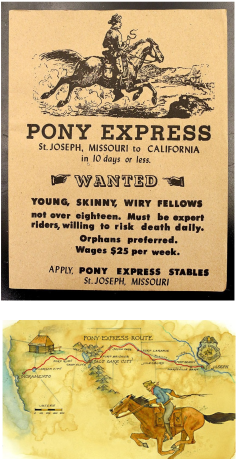
\includegraphics[width=6cm]{docs/pony-express.png}
      \caption{A job application poster and a relay route used for the Pony Express. 
      Images taken from \cite{orphans} and \cite{ponyroute} respectively.}
  \end{center}
\end{wrapfigure}

A system of using relays for delivering packages is not a particularly new idea. A 
famous (and shortlived!) example of such a relay system was the Pony Express company which 
was used a system of a relay of horse riders tp transport mail from St. Joseph, Missouri to 
Sacramento, California. 

To quote the Wikipedia article

\begin{quote}
\textit{``Operated by Central Overland California and Pike's Peak Express Company, the Pony Express was a great 
financial investment to the U.S. During its 18 months of operation, it reduced the time for messages to travel 
between the Atlantic and Pacific coasts to about 10 days. It became the West's most direct means of east-west 
communication before the transcontinental telegraph was established (October 24, 1861), and was vital for tying 
the new U.S. state of California with the rest of the United States.The Pony Express demonstrated that a unified 
transcontinental system of communications could be established and operated year-round. ''}
\end{quote}


While the invention of the telegraph might have run the Pony Express out of business, the idea of using relay agents 
such as drones --- instead of horses! --- to transfer packages can have applications today for sending physical goods 
(which of course can't be telegraphed! \Winkey) such as  life-saving medicinces in under-developed 
countries or in disaster relief areas. 
ZipLine\cite{zipline} \cite{zipline-ted} and Matternet \cite{matternet} are just two of the companies which 
are involved in building networks of drones for precisely such missions.

\begin{figure}[H]
  \centering
  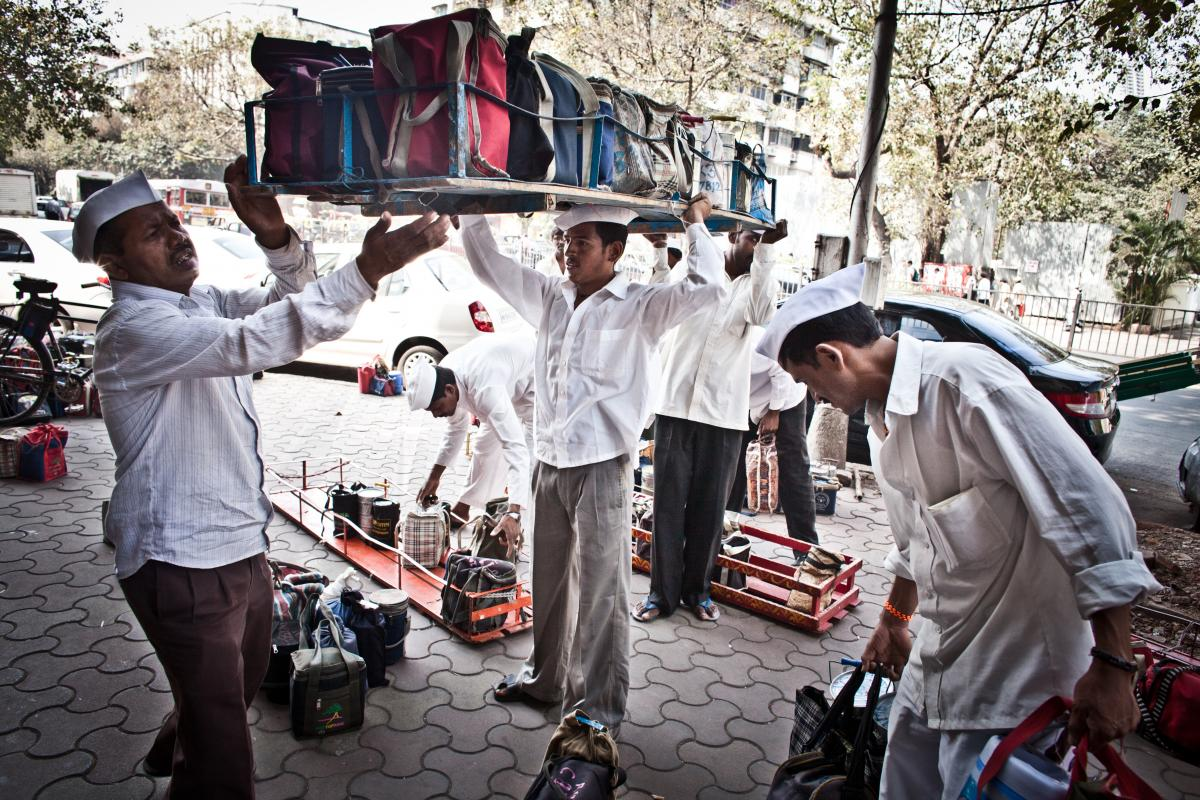
\includegraphics[width=12cm]{docs/dabba.jpg}
  \caption{Dabbawallas exchanging lunchboxes (dabbas) at a relay point. Image from \cite{Magazine2019Oct} }
\end{figure}

Another relay system for package deliveries (135 years old and still functioning!) is that of 
the \textit{dabbawallas} \footnote{literally: lunchbox carriers} used for transporting lunch boxes from 
homes and restaurants to people at work in Mumbai, India. To quote from \cite{dabba}
\begin{quote}
\textit{Four thousand five hundred semi-literate dabbawalas collect and deliver 175,000 packages 
within hours. What should we learn from this unique, simple and highly efficient 120-year-old 
logistics system? [\ldots] After the customer leaves for work, her lunch is packed into a tiffin 
provided by the dabbawala. A color-coded notation on the handle identifies its owner and destination. 
Once the dabbawala has picked up the tiffin, he moves fast using a combination of bicycles, trains and his 
two feet.}

\textit{A BBC crew filming dabbawalas in action was amazed at their speed. ``Following our dabbawala 
wasn't easy, our film crew quickly lost him in the congestion of the train station. At Victoria 
Terminus we found other fast moving dabbawalas, but not our subject... and at Mr Bhapat's ayurvedic 
pharmacy, the lunch had arrived long before the film crew,'' the documentary noted wryly. So, how do 
they work so efficiently?}

\textit{The entire system depends on teamwork and meticulous timing. Tiffins are collected from homes 
between 7.00 am and 9.00 am, and taken to the nearest railway station. At various intermediary stations, 
they are hauled onto platforms and sorted out for area-wise distribution, so that a single tiffin could 
change hands three to four times in the course of its daily journey.}

\textit{At Mumbai's downtown stations, the last link in the chain, a final relay of dabbawalas fan 
out to the tiffins' destined bellies. Lunch hour over, the whole process moves into reverse and the 
tiffins return to suburban homes by 6.00 pm.}
\end{quote}

See \url{https://youtu.be/dX-0el2wuEU} for a short video on the dabbawallas. 


\chapter{\texttt{README.md}}

This \verb|README| file can be read more clearly alongside its appropriate formatting at \\
\url{https://github.com/gtelang/PackageHandoff_Python/tree/master/packagehandoff_lit}

\begin{flushleft} \small\label{scrap30}\raggedright\small
\NWtarget{nuweb27}{} \verb@"README.md"@\nobreak\ {\footnotesize {27}}$\equiv$
\vspace{-1ex}
\begin{list}{}{} \item
\mbox{}\verb@    @\\
\mbox{}\verb@To run this code, you will need a distribution of Python 2.7.12 along @\\
\mbox{}\verb@with the following libraries@\\
\mbox{}\verb@@\\
\mbox{}\verb@- networkx@\\
\mbox{}\verb@- matplotlib@\\
\mbox{}\verb@- numpy @\\
\mbox{}\verb@- scipy@\\
\mbox{}\verb@- cgal-bindings@\\
\mbox{}\verb@- cvxpy@\\
\mbox{}\verb@@\\
\mbox{}\verb@All source code is contained in the .web file. If you modify the file, the @\\
\mbox{}\verb@resulting code and corresponding description file can be weaved and tangled @\\
\mbox{}\verb@with the script `weave-tangle.sh`. You will need the @\\
\mbox{}\verb@@\\
\mbox{}\verb@- [pdflatex](https://linux.die.net/man/1/pdflatex)@\\
\mbox{}\verb@- [nuweb](http://nuweb.sourceforge.net/) @\\
\mbox{}\verb@- [asymptote](http://asymptote.sourceforge.net/) @\\
\mbox{}\verb@  @\\
\mbox{}\verb@executables to be somewhere on your system's path. @\\
\mbox{}\verb@@\\
\mbox{}\verb@All source code is in the `src' directory. The asy2d, asy3d and docs@\\
\mbox{}\verb@folders can be neglected since they contain images and documents @\\
\mbox{}\verb@referenced in the `packagehandoff.pdf' file. From the point of view of @\\
\mbox{}\verb@_running_ the code they can be ignored. @\\
\mbox{}\verb@@\\
\mbox{}\verb@@\\
\mbox{}\verb@@\\
\mbox{}\verb@@{\NWsep}
\end{list}
\vspace{-1.5ex}
\footnotesize
\begin{list}{}{\setlength{\itemsep}{-\parsep}\setlength{\itemindent}{-\leftmargin}}

\item{}
\end{list}
\vspace{4ex}
\end{flushleft}
\chapter{\texttt{utils\char`_graphics.py}}

This file contains useful functions for visualization and plotting functions described in the previous chapters.
%{python-mode}%
\begin{flushleft} \small\label{scrap31}\raggedright\small
\NWtarget{nuweb28}{} \verb@"src/utils_graphics.py"@\nobreak\ {\footnotesize {28}}$\equiv$
\vspace{-1ex}
\begin{list}{}{} \item
\mbox{}\verb@    @\\
\mbox{}\verb@from matplotlib import rc@\\
\mbox{}\verb@from colorama import Fore@\\
\mbox{}\verb@from colorama import Style@\\
\mbox{}\verb@from scipy.optimize import minimize@\\
\mbox{}\verb@from sklearn.cluster import KMeans@\\
\mbox{}\verb@import argparse@\\
\mbox{}\verb@import itertools@\\
\mbox{}\verb@import math@\\
\mbox{}\verb@import matplotlib as mpl@\\
\mbox{}\verb@import matplotlib.pyplot as plt@\\
\mbox{}\verb@import numpy as np@\\
\mbox{}\verb@import os@\\
\mbox{}\verb@import pprint as pp@\\
\mbox{}\verb@import randomcolor @\\
\mbox{}\verb@import sys@\\
\mbox{}\verb@import time@\\
\mbox{}\verb@@\\
\mbox{}\verb@xlim, ylim = [0,1], [0,1]@\\
\mbox{}\verb@@\\
\mbox{}\verb@# Borrowed from https://stackoverflow.com/a/9701141@\\
\mbox{}\verb@import numpy as np@\\
\mbox{}\verb@import colorsys@\\
\mbox{}\verb@@\\
\mbox{}\verb@def get_colors(num_colors, lightness=0.2):@\\
\mbox{}\verb@    colors=[]@\\
\mbox{}\verb@    for i in np.arange(60., 360., 300. / num_colors):@\\
\mbox{}\verb@        hue        = i/360.0@\\
\mbox{}\verb@        saturation = 0.95@\\
\mbox{}\verb@        colors.append(colorsys.hls_to_rgb(hue, lightness, saturation))@\\
\mbox{}\verb@    return colors@\\
\mbox{}\verb@@{\NWsep}
\end{list}
\vspace{-1.5ex}
\footnotesize
\begin{list}{}{\setlength{\itemsep}{-\parsep}\setlength{\itemindent}{-\leftmargin}}

\item{}
\end{list}
\vspace{4ex}
\end{flushleft}
%{/python-mode}%

\newpage

\chapter{\texttt{utils\char`_algo.py}}

This file contains useful functions for writing algorithms described in the previous chapters.

%{python-mode}%
\begin{flushleft} \small\label{scrap32}\raggedright\small
\NWtarget{nuweb29}{} \verb@"src/utils_algo.py"@\nobreak\ {\footnotesize {29}}$\equiv$
\vspace{-1ex}
\begin{list}{}{} \item
\mbox{}\verb@@\\
\mbox{}\verb@import numpy as np@\\
\mbox{}\verb@import random@\\
\mbox{}\verb@from colorama import Fore@\\
\mbox{}\verb@from colorama import Style@\\
\mbox{}\verb@@\\
\mbox{}\verb@def vector_chain_from_point_list(pts):@\\
\mbox{}\verb@    vec_chain = []@\\
\mbox{}\verb@    for pair in zip(pts, pts[1:]):@\\
\mbox{}\verb@        tail= np.array (pair[0])@\\
\mbox{}\verb@        head= np.array (pair[1])@\\
\mbox{}\verb@        vec_chain.append(head-tail)@\\
\mbox{}\verb@@\\
\mbox{}\verb@    return vec_chain@\\
\mbox{}\verb@@\\
\mbox{}\verb@def length_polygonal_chain(pts):@\\
\mbox{}\verb@    vec_chain = vector_chain_from_point_list(pts)@\\
\mbox{}\verb@@\\
\mbox{}\verb@    acc = 0@\\
\mbox{}\verb@    for vec in vec_chain:@\\
\mbox{}\verb@        acc = acc + np.linalg.norm(vec)@\\
\mbox{}\verb@    return acc@\\
\mbox{}\verb@def pointify_vector (x):@\\
\mbox{}\verb@    if len(x) % 2 == 0:@\\
\mbox{}\verb@        pts = []@\\
\mbox{}\verb@        for i in range(len(x))[::2]:@\\
\mbox{}\verb@            pts.append( [x[i],x[i+1]] )@\\
\mbox{}\verb@        return pts@\\
\mbox{}\verb@    else :@\\
\mbox{}\verb@        sys.exit('List of items does not have an even length to be able to be pointifyed')@\\
\mbox{}\verb@def flatten_list_of_lists(l):@\\
\mbox{}\verb@       return [item for sublist in l for item in sublist]@\\
\mbox{}\verb@def print_list(xs):@\\
\mbox{}\verb@    for x in xs:@\\
\mbox{}\verb@        print x@\\
\mbox{}\verb@def partial_sums( xs ):@\\
\mbox{}\verb@    psum = 0@\\
\mbox{}\verb@    acc = []@\\
\mbox{}\verb@    for x in xs:@\\
\mbox{}\verb@        psum = psum+x@\\
\mbox{}\verb@        acc.append( psum )@\\
\mbox{}\verb@    return acc@\\
\mbox{}\verb@def are_site_orderings_equal(sites1, sites2):@\\
\mbox{}\verb@@\\
\mbox{}\verb@    for (x1,y1), (x2,y2) in zip(sites1, sites2): @\\
\mbox{}\verb@        if (x1-x2)**2 + (y1-y2)**2 > 1e-8:@\\
\mbox{}\verb@            return False@\\
\mbox{}\verb@    return True@\\
\mbox{}\verb@def bunch_of_non_uniform_random_points(numpts):@\\
\mbox{}\verb@    cluster_size = int(np.sqrt(numpts)) @\\
\mbox{}\verb@    numcenters   = cluster_size@\\
\mbox{}\verb@    @\\
\mbox{}\verb@    import scipy@\\
\mbox{}\verb@    import random@\\
\mbox{}\verb@    centers = scipy.rand(numcenters,2).tolist()@\\
\mbox{}\verb@@\\
\mbox{}\verb@    scale, points = 4.0, []@\\
\mbox{}\verb@    for c in centers:@\\
\mbox{}\verb@        cx, cy = c[0], c[1]@\\
\mbox{}\verb@        # For current center $c$ of this loop, generate \verb|cluster_size| points uniformly in a square centered at it@\\
\mbox{}\verb@           @\\
\mbox{}\verb@        sq_size      = min(cx,1-cx,cy, 1-cy)@\\
\mbox{}\verb@        loc_pts_x    = np.random.uniform(low=cx-sq_size/scale, high=cx+sq_size/scale, size=(cluster_size,))@\\
\mbox{}\verb@        loc_pts_y    = np.random.uniform(low=cy-sq_size/scale, high=cy+sq_size/scale, size=(cluster_size,))@\\
\mbox{}\verb@        points.extend(zip(loc_pts_x, loc_pts_y))@\\
\mbox{}\verb@        @\\
\mbox{}\verb@@\\
\mbox{}\verb@    # Whatever number of points are left to be generated, generate them uniformly inside the unit-square@\\
\mbox{}\verb@       @\\
\mbox{}\verb@    num_remaining_pts = numpts - cluster_size * numcenters@\\
\mbox{}\verb@    remaining_pts = scipy.rand(num_remaining_pts, 2).tolist()@\\
\mbox{}\verb@    points.extend(remaining_pts)@\\
\mbox{}\verb@    @\\
\mbox{}\verb@@\\
\mbox{}\verb@    return points@\\
\mbox{}\verb@    @\\
\mbox{}\verb@def write_to_yaml_file(data, dir_name, file_name):@\\
\mbox{}\verb@   import yaml@\\
\mbox{}\verb@   with open(dir_name + '/' + file_name, 'w') as outfile:@\\
\mbox{}\verb@     yaml.dump( data, outfile, default_flow_style = False)@\\
\mbox{}\verb@@{\NWsep}
\end{list}
\vspace{-1.5ex}
\footnotesize
\begin{list}{}{\setlength{\itemsep}{-\parsep}\setlength{\itemindent}{-\leftmargin}}

\item{}
\end{list}
\vspace{4ex}
\end{flushleft}
%{/python-mode}%

\chapter{Implementation of \textlangle \texttt{Run Handlers}\textrangle}

This chunk contains code required for the interactive input of sites and agents onto the canvas. 

%{python-mode}%
\begin{flushleft} \small\label{scrap33}\raggedright\small
\NWtarget{nuweb31}{} $\langle\,${\itshape Run Handlers}\nobreak\ {\footnotesize {31}}$\,\rangle\equiv$
\vspace{-1ex}
\begin{list}{}{} \item
\mbox{}\verb@@\\
\mbox{}\verb@# Set up logging information relevant to this module@\\
\mbox{}\verb@logger=logging.getLogger(__name__)@\\
\mbox{}\verb@logging.basicConfig(level=logging.DEBUG)@\\
\mbox{}\verb@@\\
\mbox{}\verb@def debug(msg):@\\
\mbox{}\verb@    frame,filename,line_number,function_name,lines,index=inspect.getouterframes(@\\
\mbox{}\verb@        inspect.currentframe())[1]@\\
\mbox{}\verb@    line=lines[0]@\\
\mbox{}\verb@    indentation_level=line.find(line.lstrip())@\\
\mbox{}\verb@    logger.debug('{i} [{m}]'.format(@\\
\mbox{}\verb@        i='.'*indentation_level, m=msg))@\\
\mbox{}\verb@@\\
\mbox{}\verb@@\\
\mbox{}\verb@def info(msg):@\\
\mbox{}\verb@    frame,filename,line_number,function_name,lines,index=inspect.getouterframes(@\\
\mbox{}\verb@        inspect.currentframe())[1]@\\
\mbox{}\verb@    line=lines[0]@\\
\mbox{}\verb@    indentation_level=line.find(line.lstrip())@\\
\mbox{}\verb@    logger.info('{i} [{m}]'.format(@\\
\mbox{}\verb@        i='.'*indentation_level, m=msg))@\\
\mbox{}\verb@@\\
\mbox{}\verb@xlim, ylim = [0,1], [0,1]@\\
\mbox{}\verb@@\\
\mbox{}\verb@def applyAxCorrection(ax):@\\
\mbox{}\verb@      ax.set_xlim([xlim[0], xlim[1]])@\\
\mbox{}\verb@      ax.set_ylim([ylim[0], ylim[1]])@\\
\mbox{}\verb@      ax.set_aspect(1.0)@\\
\mbox{}\verb@@\\
\mbox{}\verb@def clearPatches(ax):@\\
\mbox{}\verb@    # Get indices cooresponding to the polygon patches@\\
\mbox{}\verb@    for index , patch in zip(range(len(ax.patches)), ax.patches):@\\
\mbox{}\verb@        if isinstance(patch, mpl.patches.Polygon) == True:@\\
\mbox{}\verb@            patch.remove()@\\
\mbox{}\verb@    ax.lines[:]=[]@\\
\mbox{}\verb@    applyAxCorrection(ax)@\\
\mbox{}\verb@@\\
\mbox{}\verb@def clearAxPolygonPatches(ax):@\\
\mbox{}\verb@@\\
\mbox{}\verb@    # Get indices cooresponding to the polygon patches@\\
\mbox{}\verb@    for index , patch in zip(range(len(ax.patches)), ax.patches):@\\
\mbox{}\verb@        if isinstance(patch, mpl.patches.Polygon) == True:@\\
\mbox{}\verb@            patch.remove()@\\
\mbox{}\verb@    ax.lines[:]=[]@\\
\mbox{}\verb@    applyAxCorrection(ax)@\\
\mbox{}\verb@@\\
\mbox{}\verb@class Single_PHO_Input:@\\
\mbox{}\verb@    def __init__(self, drone_info = [] , source = None, target=None):@\\
\mbox{}\verb@           self.drone_info = drone_info @\\
\mbox{}\verb@           self.source     = source@\\
\mbox{}\verb@           self.target     = target@\\
\mbox{}\verb@@\\
\mbox{}\verb@    def get_drone_pis (self):@\\
\mbox{}\verb@           return [self.drone_info[idx][0] for idx in range(len(self.drone_info)) ]@\\
\mbox{}\verb@           @\\
\mbox{}\verb@    def get_drone_uis (self):@\\
\mbox{}\verb@           return [self.drone_info[idx][1] for idx in range(len(self.drone_info)) ]@\\
\mbox{}\verb@         @\\
\mbox{}\verb@    def get_tour(self, algo, plot_tour_p=False):@\\
\mbox{}\verb@           return algo( self.drone_info, @\\
\mbox{}\verb@                        self.source, @\\
\mbox{}\verb@                        self.target, @\\
\mbox{}\verb@                        plot_tour_p    )@\\
\mbox{}\verb@@\\
\mbox{}\verb@    # Methods for \verb|ReverseHorseflyInput|@\\
\mbox{}\verb@    def clearAllStates (self):@\\
\mbox{}\verb@          self.drone_info = []@\\
\mbox{}\verb@          self.source = None@\\
\mbox{}\verb@          self.target = None@\\
\mbox{}\verb@@\\
\mbox{}\verb@def single_pho_run_handler():@\\
\mbox{}\verb@    import random@\\
\mbox{}\verb@    def wrapperEnterRunPoints(fig, ax, run):@\\
\mbox{}\verb@      def _enterPoints(event):@\\
\mbox{}\verb@        if event.name      == 'button_press_event'          and \@\\
\mbox{}\verb@           (event.button   == 1 or event.button == 3)       and \@\\
\mbox{}\verb@            event.dblclick == True and event.xdata  != None and event.ydata  != None:@\\
\mbox{}\verb@@\\
\mbox{}\verb@             if event.button == 1:  @\\
\mbox{}\verb@                 # Insert blue circle representing the initial position of a drone@\\
\mbox{}\verb@                 print Fore.GREEN@\\
\mbox{}\verb@                 newPoint = (event.xdata, event.ydata)@\\
\mbox{}\verb@                 speed    = np.random.uniform() # float(raw_input('What speed do you want for the drone at '+str(newPoint)))@\\
\mbox{}\verb@                 run.drone_info.append( (newPoint, speed) ) @\\
\mbox{}\verb@                 patchSize  = (xlim[1]-xlim[0])/40.0@\\
\mbox{}\verb@                 print Style.RESET_ALL@\\
\mbox{}\verb@                 @\\
\mbox{}\verb@                 ax.add_patch( mpl.patches.Circle( newPoint, radius = patchSize,@\\
\mbox{}\verb@                                                   facecolor='#b7e8cc', edgecolor='black'  ))@\\
\mbox{}\verb@@\\
\mbox{}\verb@                 ax.text( newPoint[0], newPoint[1], "{:.2f}".format(speed), fontsize=15, @\\
\mbox{}\verb@                          horizontalalignment='center', verticalalignment='center' )@\\
\mbox{}\verb@@\\
\mbox{}\verb@                 ax.set_title('Number of drones inserted: ' +\@\\
\mbox{}\verb@                              str(len(run.drone_info)), fontdict={'fontsize':25})@\\
\mbox{}\verb@                 @\\
\mbox{}\verb@             elif event.button == 3:  @\\
\mbox{}\verb@                 # Insert big red circles representing the source and target points@\\
\mbox{}\verb@                 patchSize  = (xlim[1]-xlim[0])/50.0@\\
\mbox{}\verb@                 if run.source is None:    @\\
\mbox{}\verb@                      run.source = (event.xdata, event.ydata)  @\\
\mbox{}\verb@                      ax.add_patch( mpl.patches.Circle( run.source, radius = patchSize, @\\
\mbox{}\verb@                                                        facecolor= '#ffd9d6', edgecolor='black', lw=1.0 ))@\\
\mbox{}\verb@                      ax.text( run.source[0], run.source[1], 'S', fontsize=15, @\\
\mbox{}\verb@                               horizontalalignment='center', verticalalignment='center' )@\\
\mbox{}\verb@@\\
\mbox{}\verb@                 elif run.target is None:@\\
\mbox{}\verb@                      run.target = (event.xdata, event.ydata)  @\\
\mbox{}\verb@                      ax.add_patch( mpl.patches.Circle( run.target, radius = patchSize, @\\
\mbox{}\verb@                                                       facecolor= '#ffd9d6', edgecolor='black', lw=1.0 ))@\\
\mbox{}\verb@                      ax.text( run.target[0], run.target[1], 'T', fontsize=15, @\\
\mbox{}\verb@                               horizontalalignment='center', verticalalignment='center' )@\\
\mbox{}\verb@                 else:@\\
\mbox{}\verb@                       print Fore.RED, "Source and Target already set", Style.RESET_ALL@\\
\mbox{}\verb@             # Clear polygon patches and set up last minute \verb|ax| tweaks@\\
\mbox{}\verb@             clearAxPolygonPatches(ax)@\\
\mbox{}\verb@             applyAxCorrection(ax)@\\
\mbox{}\verb@             fig.canvas.draw()@\\
\mbox{}\verb@      return _enterPoints@\\
\mbox{}\verb@@\\
\mbox{}\verb@    # The key-stack argument is mutable! I am using this hack to my advantage.@\\
\mbox{}\verb@    def wrapperkeyPressHandler(fig, ax, run): @\\
\mbox{}\verb@           def _keyPressHandler(event):@\\
\mbox{}\verb@               if event.key in ['i', 'I']:  @\\
\mbox{}\verb@@\\
\mbox{}\verb@                    # Select algorithm to execute@\\
\mbox{}\verb@                    algo_str = raw_input(Fore.YELLOW                                             +\@\\
\mbox{}\verb@                            "Enter algorithm to be used to compute the tour:\n Options are:\n"   +\@\\
\mbox{}\verb@                            " (odw)     One Dimensional Wavefront \n"                            +\@\\
\mbox{}\verb@                            Style.RESET_ALL)@\\
\mbox{}\verb@@\\
\mbox{}\verb@                    algo_str = algo_str.lstrip()@\\
\mbox{}\verb@                     @\\
\mbox{}\verb@                    # Incase there are patches present from the previous clustering, just clear them@\\
\mbox{}\verb@                    clearAxPolygonPatches(ax)@\\
\mbox{}\verb@                    if   algo_str == 'odw':@\\
\mbox{}\verb@                          tour = run.get_tour( algo_odw, plot_tour_p=True )@\\
\mbox{}\verb@                    else:@\\
\mbox{}\verb@                          print "Unknown option. No horsefly for you! ;-D "@\\
\mbox{}\verb@                          sys.exit()@\\
\mbox{}\verb@                    applyAxCorrection(ax)@\\
\mbox{}\verb@                    fig.canvas.draw()@\\
\mbox{}\verb@                    @\\
\mbox{}\verb@               elif event.key in ['c', 'C']: @\\
\mbox{}\verb@                    # Clear canvas and states of all objects@\\
\mbox{}\verb@                    run.clearAllStates()@\\
\mbox{}\verb@                    ax.cla()@\\
\mbox{}\verb@                                  @\\
\mbox{}\verb@                    applyAxCorrection(ax)@\\
\mbox{}\verb@                    ax.set_xticks([])@\\
\mbox{}\verb@                    ax.set_yticks([])@\\
\mbox{}\verb@                                     @\\
\mbox{}\verb@                    fig.texts = []@\\
\mbox{}\verb@                    fig.canvas.draw()@\\
\mbox{}\verb@           return _keyPressHandler@\\
\mbox{}\verb@    @\\
\mbox{}\verb@    # Set up interactive canvas@\\
\mbox{}\verb@    fig, ax =  plt.subplots()@\\
\mbox{}\verb@    run = Single_PHO_Input()@\\
\mbox{}\verb@        @\\
\mbox{}\verb@    from matplotlib import rc@\\
\mbox{}\verb@    @\\
\mbox{}\verb@    # specify the custom font to use@\\
\mbox{}\verb@    plt.rcParams['font.family'] = 'sans-serif'@\\
\mbox{}\verb@    plt.rcParams['font.sans-serif'] = 'Times New Roman'@\\
\mbox{}\verb@@\\
\mbox{}\verb@    xlim = utils_graphics.xlim@\\
\mbox{}\verb@    ylim = utils_graphics.ylim@\\
\mbox{}\verb@@\\
\mbox{}\verb@    ax.set_xlim([xlim[0], xlim[1]])@\\
\mbox{}\verb@    ax.set_ylim([ylim[0], ylim[1]])@\\
\mbox{}\verb@    ax.set_aspect(1.0)@\\
\mbox{}\verb@    ax.set_xticks([])@\\
\mbox{}\verb@    ax.set_yticks([])@\\
\mbox{}\verb@          @\\
\mbox{}\verb@    ax.set_title("Enter drone positions, source and target onto canvas. \n \@\\
\mbox{}\verb@(Enter speeds into the terminal, after inserting a drone at a particular position)")@\\
\mbox{}\verb@@\\
\mbox{}\verb@    mouseClick   = wrapperEnterRunPoints (fig,ax, run)@\\
\mbox{}\verb@    fig.canvas.mpl_connect('button_press_event' , mouseClick)@\\
\mbox{}\verb@          @\\
\mbox{}\verb@    keyPress     = wrapperkeyPressHandler(fig,ax, run)@\\
\mbox{}\verb@    fig.canvas.mpl_connect('key_press_event', keyPress   )@\\
\mbox{}\verb@    @\\
\mbox{}\verb@    plt.show()@\\
\mbox{}\verb@@\\
\mbox{}\verb@@\\
\mbox{}\verb@@\\
\mbox{}\verb@@\\
\mbox{}\verb@@\\
\mbox{}\verb@class Multiple_PHO_Input:@\\
\mbox{}\verb@    def __init__(self, drone_info = [] , sources = [], targets=[]):@\\
\mbox{}\verb@           self.drone_info = drone_info @\\
\mbox{}\verb@           self.sources     = sources@\\
\mbox{}\verb@           self.targets     = targets@\\
\mbox{}\verb@@\\
\mbox{}\verb@    def get_drone_pis (self):@\\
\mbox{}\verb@           return [self.drone_info[idx][0] for idx in range(len(self.drone_info)) ]@\\
\mbox{}\verb@           @\\
\mbox{}\verb@    def get_drone_uis (self):@\\
\mbox{}\verb@           return [self.drone_info[idx][1] for idx in range(len(self.drone_info)) ]@\\
\mbox{}\verb@         @\\
\mbox{}\verb@    def get_tour(self, algo, plot_tour_p=False):@\\
\mbox{}\verb@           return algo( self.drone_info, @\\
\mbox{}\verb@                        self.sources, @\\
\mbox{}\verb@                        self.targets, @\\
\mbox{}\verb@                        plot_tour_p    )@\\
\mbox{}\verb@@\\
\mbox{}\verb@    # Methods for \verb|ReverseHorseflyInput|@\\
\mbox{}\verb@    def clearAllStates (self):@\\
\mbox{}\verb@          self.drone_info = []@\\
\mbox{}\verb@          self.sources = []@\\
\mbox{}\verb@          self.targets = []@\\
\mbox{}\verb@@\\
\mbox{}\verb@@\\
\mbox{}\verb@# distinct colors, obtained from https://sashat.me/2017/01/11/list-of-20-simple-distinct-colors/@\\
\mbox{}\verb@cols = ['#e6194b', '#3cb44b', '#ffe119', '#4363d8', '#f58231', @\\
\mbox{}\verb@        '#911eb4', '#46f0f0', '#f032e6', '#bcf60c', '#fabebe', @\\
\mbox{}\verb@        '#008080', '#e6beff', '#9a6324', '#fffac8', '#800000', @\\
\mbox{}\verb@        '#aaffc3', '#808000', '#ffd8b1', '#000075', '#808080'] @\\
\mbox{}\verb@@\\
\mbox{}\verb@@\\
\mbox{}\verb@numrobscanvas = 0@\\
\mbox{}\verb@@\\
\mbox{}\verb@def multiple_pho_run_handler():@\\
\mbox{}\verb@    import random@\\
\mbox{}\verb@    def wrapperEnterRunPoints(fig, ax, run):@\\
\mbox{}\verb@      def _enterPoints(event):@\\
\mbox{}\verb@        if event.name      == 'button_press_event'          and \@\\
\mbox{}\verb@           (event.button   == 1 or event.button == 3)       and \@\\
\mbox{}\verb@            event.dblclick == True and event.xdata  != None and event.ydata  != None:@\\
\mbox{}\verb@@\\
\mbox{}\verb@             if event.button == 1:  @\\
\mbox{}\verb@                 # Insert circle representing the initial position of a drone@\\
\mbox{}\verb@                 print Fore.GREEN@\\
\mbox{}\verb@                 newPoint = (event.xdata, event.ydata)@\\
\mbox{}\verb@                 speed    = np.random.uniform() # float(raw_input('What speed do you want for the drone at '+str(newPoint)))@\\
\mbox{}\verb@                 run.drone_info.append( (newPoint, speed) ) @\\
\mbox{}\verb@                 patchSize  = (xlim[1]-xlim[0])/20.0@\\
\mbox{}\verb@                 print Style.RESET_ALL@\\
\mbox{}\verb@                 @\\
\mbox{}\verb@                 global numrobscanvas@\\
\mbox{}\verb@                 ax.add_patch( mpl.patches.Circle( newPoint, radius = patchSize,@\\
\mbox{}\verb@                                                   facecolor='#EBEBEB', edgecolor='black'  ))@\\
\mbox{}\verb@@\\
\mbox{}\verb@                 ax.text( newPoint[0], newPoint[1], "{:.2f}".format(speed) + "\n" + str(numrobscanvas) , fontsize=10, @\\
\mbox{}\verb@                          horizontalalignment='center', verticalalignment='center' )@\\
\mbox{}\verb@@\\
\mbox{}\verb@                 numrobscanvas += 1    @\\
\mbox{}\verb@                 ax.set_title('Number of drones inserted: ' +\@\\
\mbox{}\verb@                              str(len(run.drone_info)), fontdict={'fontsize':25})@\\
\mbox{}\verb@                 @\\
\mbox{}\verb@             elif event.button == 3:  @\\
\mbox{}\verb@                 # Insert big colored circles representing the source and target points@\\
\mbox{}\verb@@\\
\mbox{}\verb@                 patchSize  = (xlim[1]-xlim[0])/30.0@\\
\mbox{}\verb@                 if (len(run.sources) + len(run.targets)) % 2 == 0 : @\\
\mbox{}\verb@                        run.sources.append((event.xdata, event.ydata))@\\
\mbox{}\verb@                        ax.add_patch( mpl.patches.Circle( run.sources[-1], radius = patchSize, @\\
\mbox{}\verb@                                                   facecolor= cols[len(run.sources) % len(cols)], edgecolor='black', lw=1.0 ))@\\
\mbox{}\verb@                        ax.text( run.sources[-1][0], run.sources[-1][1], 'S'+str(len(run.sources)-1), fontsize=15, @\\
\mbox{}\verb@                                 horizontalalignment='center', verticalalignment='center' )@\\
\mbox{}\verb@@\\
\mbox{}\verb@                 else :@\\
\mbox{}\verb@                      run.targets.append((event.xdata, event.ydata))@\\
\mbox{}\verb@                      ax.add_patch( mpl.patches.Circle( run.targets[-1], radius = patchSize, @\\
\mbox{}\verb@                                                       facecolor= cols[len(run.sources)%len(cols)], edgecolor='black', lw=1.0 ))@\\
\mbox{}\verb@                      ax.text( run.targets[-1][0], run.targets[-1][1], 'T'+str(len(run.targets)-1), fontsize=15, @\\
\mbox{}\verb@                               horizontalalignment='center', verticalalignment='center' )@\\
\mbox{}\verb@@\\
\mbox{}\verb@             # Clear polygon patches and set up last minute \verb|ax| tweaks@\\
\mbox{}\verb@             clearAxPolygonPatches(ax)@\\
\mbox{}\verb@             applyAxCorrection(ax)@\\
\mbox{}\verb@             fig.canvas.draw()@\\
\mbox{}\verb@      return _enterPoints@\\
\mbox{}\verb@@\\
\mbox{}\verb@    # The key-stack argument is mutable! I am using this hack to my advantage.@\\
\mbox{}\verb@    def wrapperkeyPressHandler(fig, ax, run): @\\
\mbox{}\verb@           def _keyPressHandler(event):@\\
\mbox{}\verb@               if event.key in ['i', 'I']:  @\\
\mbox{}\verb@@\\
\mbox{}\verb@                    # Select algorithm to execute@\\
\mbox{}\verb@                    algo_str = raw_input(Fore.YELLOW                                             +\@\\
\mbox{}\verb@                            "Enter algorithm to be used to compute the tour:\n Options are:\n"   +\@\\
\mbox{}\verb@                            " (mm)     Match-and-move \n"                            +\@\\
\mbox{}\verb@                            Style.RESET_ALL)@\\
\mbox{}\verb@@\\
\mbox{}\verb@                    algo_str = algo_str.lstrip()@\\
\mbox{}\verb@                     @\\
\mbox{}\verb@                    # Incase there are patches present from the previous clustering, just clear them@\\
\mbox{}\verb@                    clearAxPolygonPatches(ax)@\\
\mbox{}\verb@                    if   algo_str == 'mm':@\\
\mbox{}\verb@                          tour = run.get_tour( algo_matchmove, plot_tour_p=True )@\\
\mbox{}\verb@                    else:@\\
\mbox{}\verb@                          print "Unknown option. No horsefly for you! ;-D "@\\
\mbox{}\verb@                          sys.exit()@\\
\mbox{}\verb@                    applyAxCorrection(ax)@\\
\mbox{}\verb@                    fig.canvas.draw()@\\
\mbox{}\verb@                    @\\
\mbox{}\verb@               elif event.key in ['c', 'C']: @\\
\mbox{}\verb@                    # Clear canvas and states of all objects@\\
\mbox{}\verb@                    run.clearAllStates()@\\
\mbox{}\verb@                    ax.cla()@\\
\mbox{}\verb@                                  @\\
\mbox{}\verb@                    applyAxCorrection(ax)@\\
\mbox{}\verb@                    ax.set_xticks([])@\\
\mbox{}\verb@                    ax.set_yticks([])@\\
\mbox{}\verb@                                     @\\
\mbox{}\verb@                    fig.texts = []@\\
\mbox{}\verb@@\\
\mbox{}\verb@                    global numrobscanvas@\\
\mbox{}\verb@                    numrobscanvas = 0@\\
\mbox{}\verb@                    fig.canvas.draw()@\\
\mbox{}\verb@           return _keyPressHandler@\\
\mbox{}\verb@    @\\
\mbox{}\verb@    # Set up interactive canvas@\\
\mbox{}\verb@    fig, ax =  plt.subplots()@\\
\mbox{}\verb@    run = Multiple_PHO_Input()@\\
\mbox{}\verb@        @\\
\mbox{}\verb@    from matplotlib import rc@\\
\mbox{}\verb@    @\\
\mbox{}\verb@    # specify the custom font to use@\\
\mbox{}\verb@    plt.rcParams['font.family'] = 'sans-serif'@\\
\mbox{}\verb@    plt.rcParams['font.sans-serif'] = 'Times New Roman'@\\
\mbox{}\verb@@\\
\mbox{}\verb@    xlim = utils_graphics.xlim@\\
\mbox{}\verb@    ylim = utils_graphics.ylim@\\
\mbox{}\verb@@\\
\mbox{}\verb@    ax.set_xlim([xlim[0], xlim[1]])@\\
\mbox{}\verb@    ax.set_ylim([ylim[0], ylim[1]])@\\
\mbox{}\verb@    ax.set_aspect(1.0)@\\
\mbox{}\verb@    ax.set_xticks([])@\\
\mbox{}\verb@    ax.set_yticks([])@\\
\mbox{}\verb@          @\\
\mbox{}\verb@    ax.set_title("Enter drone positions, sources and targets onto canvas.")@\\
\mbox{}\verb@@\\
\mbox{}\verb@    mouseClick   = wrapperEnterRunPoints (fig,ax, run)@\\
\mbox{}\verb@    fig.canvas.mpl_connect('button_press_event' , mouseClick)@\\
\mbox{}\verb@          @\\
\mbox{}\verb@    keyPress     = wrapperkeyPressHandler(fig,ax, run)@\\
\mbox{}\verb@    fig.canvas.mpl_connect('key_press_event', keyPress   )@\\
\mbox{}\verb@    @\\
\mbox{}\verb@    plt.show()@\\
\mbox{}\verb@@\\
\mbox{}\verb@@{\NWsep}
\end{list}
\vspace{-1.5ex}
\footnotesize
\begin{list}{}{\setlength{\itemsep}{-\parsep}\setlength{\itemindent}{-\leftmargin}}
\item \NWtxtMacroRefIn\ \NWlink{nuweb3}{3}.
\item \NWtxtIdentsUsed\nobreak\  \verb@algo_matchmove@\nobreak\ \NWlink{nuweb14a}{14a}, \verb@algo_odw@\nobreak\ \NWlink{nuweb7}{7}.
\item{}
\end{list}
\vspace{4ex}
\end{flushleft}
%{/python-mode}%

\chapter{Implementation of \textlangle\texttt{Plotting}\textrangle}

We typically plot the tours onto a separate window if the boolean switch \verb|plot_tour_p| 
is set to \verb|True| while calling the algorithm. The path of the package is shown in bold red. 
The paths of the drones from their initial positions to the point where they pick up the package 
from another drone are shown in blue.

An example output from the \verb|plot_tour| function is shown below.

\begin{figure}[H]
\centering
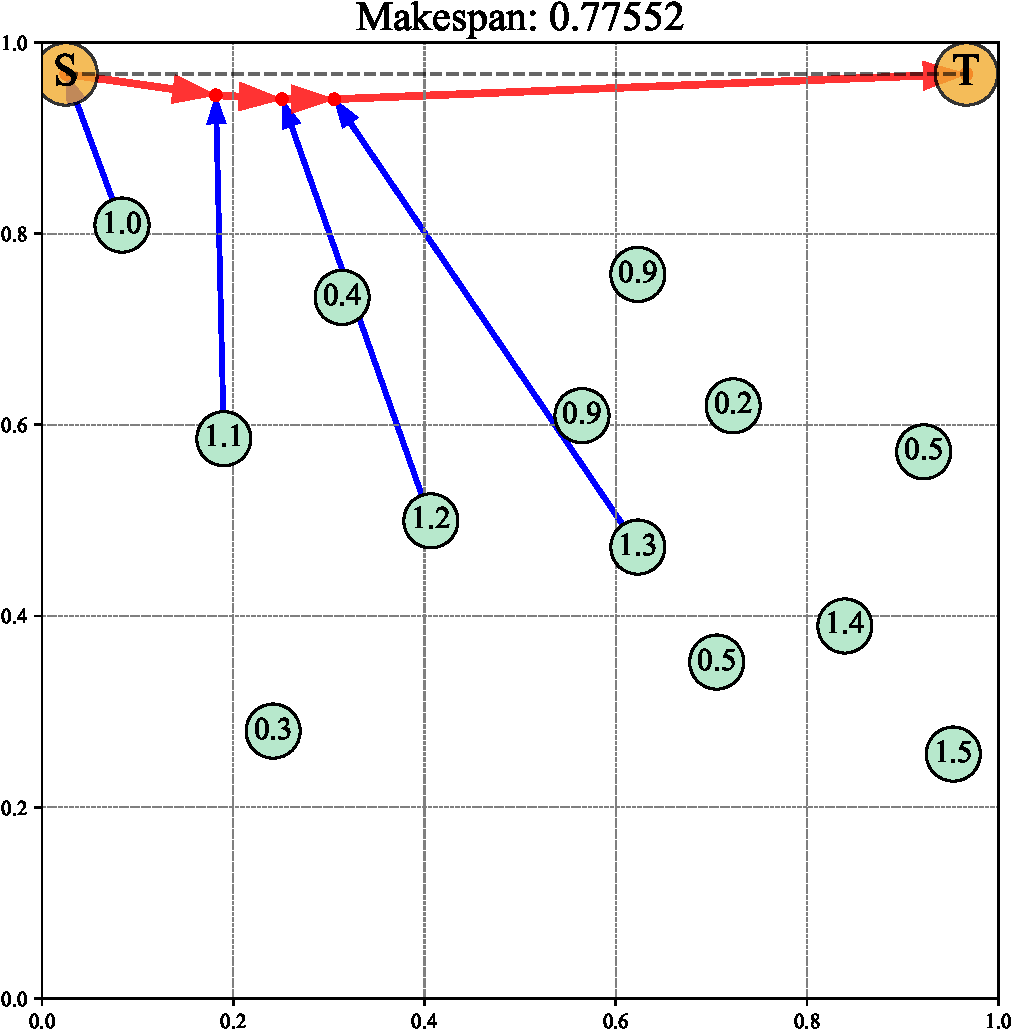
\includegraphics[width=8cm]{docs/pho_example_plot.pdf}
\caption{The numbers inside the circle indicate the speed of the drone}
\end{figure}

%{python-mode}%
\begin{flushleft} \small\label{scrap34}\raggedright\small
\NWtarget{nuweb38}{} $\langle\,${\itshape Plotting}\nobreak\ {\footnotesize {38}}$\,\rangle\equiv$
\vspace{-1ex}
\begin{list}{}{} \item
\mbox{}\verb@@\\
\mbox{}\verb@def plot_tour(fig, ax, figtitle, source, target, @\\
\mbox{}\verb@              drone_info, used_drones, package_trail,@\\
\mbox{}\verb@              xlims=[0,1],@\\
\mbox{}\verb@              ylims=[0,1],@\\
\mbox{}\verb@              aspect_ratio=1.0,@\\
\mbox{}\verb@              speedfontsize=10,@\\
\mbox{}\verb@              speedmarkersize=20,@\\
\mbox{}\verb@              sourcetargetmarkerfontsize=15,@\\
\mbox{}\verb@              sourcetargetmarkersize=20 ):@\\
\mbox{}\verb@@\\
\mbox{}\verb@    import matplotlib.ticker as ticker@\\
\mbox{}\verb@    ax.set_aspect(aspect_ratio)@\\
\mbox{}\verb@    ax.set_xlim(xlims)@\\
\mbox{}\verb@    ax.set_ylim(ylims)@\\
\mbox{}\verb@@\\
\mbox{}\verb@    plt.rc('font', family='serif')@\\
\mbox{}\verb@@\\
\mbox{}\verb@    # Draw the package trail@\\
\mbox{}\verb@    xs, ys = extract_coordinates(package_trail)@\\
\mbox{}\verb@    ax.plot(xs,ys, 'ro', markersize=5 )@\\
\mbox{}\verb@    for idx in range(len(xs)-1):@\\
\mbox{}\verb@          plt.arrow( xs[idx], ys[idx], xs[idx+1]-xs[idx], ys[idx+1]-ys[idx], @\\
\mbox{}\verb@                    **{'length_includes_head': True, @\\
\mbox{}\verb@                       'width': 0.007 , @\\
\mbox{}\verb@                       'head_width':0.025, @\\
\mbox{}\verb@                       'fc': 'r', @\\
\mbox{}\verb@                       'ec': 'none',@\\
\mbox{}\verb@                       'alpha': 0.8})@\\
\mbox{}\verb@@\\
\mbox{}\verb@@\\
\mbox{}\verb@    # Draw the source, target, and initial positions of the robots as bold dots@\\
\mbox{}\verb@    xs,ys = extract_coordinates([source, target])@\\
\mbox{}\verb@    ax.plot(xs,ys, 'o', markersize=sourcetargetmarkersize, alpha=1.0, ms=10, mec='k', mfc='#F1AB30' )@\\
\mbox{}\verb@    #ax.plot(xs,ys, 'k--', alpha=0.6 ) # light line connecting source and target@\\
\mbox{}\verb@@\\
\mbox{}\verb@    ax.text(source[0], source[1], 'S', fontsize=sourcetargetmarkerfontsize,\@\\
\mbox{}\verb@            horizontalalignment='center',verticalalignment='center')@\\
\mbox{}\verb@    ax.text(target[0], target[1], 'T', fontsize=sourcetargetmarkerfontsize,\@\\
\mbox{}\verb@            horizontalalignment='center',verticalalignment='center')@\\
\mbox{}\verb@@\\
\mbox{}\verb@    xs, ys = extract_coordinates( [ drone_info[idx][0] for idx in range(len(drone_info)) ]  )@\\
\mbox{}\verb@    ax.plot(xs,ys, 'o', markersize=speedmarkersize, alpha = 1.0, mec='None', mfc='#b7e8cc' )@\\
\mbox{}\verb@@\\
\mbox{}\verb@    # Draw speed labels@\\
\mbox{}\verb@    for idx in range(len(drone_info)):@\\
\mbox{}\verb@         ax.text( drone_info[idx][0][0], drone_info[idx][0][1], format(drone_info[idx][1],'.2f'),@\\
\mbox{}\verb@                  fontsize=speedfontsize, horizontalalignment='center', verticalalignment='center' )@\\
\mbox{}\verb@@\\
\mbox{}\verb@    # Draw drone path from initial position to interception point@\\
\mbox{}\verb@    for pt, idx in zip(package_trail, used_drones):@\\
\mbox{}\verb@         initdroneposn = drone_info[idx][0]@\\
\mbox{}\verb@         handoffpoint  = pt@\\
\mbox{}\verb@    @\\
\mbox{}\verb@         xs, ys = extract_coordinates([initdroneposn, handoffpoint])@\\
\mbox{}\verb@         plt.arrow( xs[0], ys[0], xs[1]-xs[0], ys[1]-ys[0], @\\
\mbox{}\verb@                    **{'length_includes_head': True, @\\
\mbox{}\verb@                       'width': 0.005 , @\\
\mbox{}\verb@                       'head_width':0.02, @\\
\mbox{}\verb@                       'fc': 'b', @\\
\mbox{}\verb@                       'ec': 'none'})@\\
\mbox{}\verb@@\\
\mbox{}\verb@    fig.suptitle(figtitle, fontsize=15)@\\
\mbox{}\verb@    ax.set_title('\nMakespan: ' + format(makespan(drone_info, used_drones, package_trail),'.5f'), fontsize=16)@\\
\mbox{}\verb@@\\
\mbox{}\verb@    startx, endx = ax.get_xlim()@\\
\mbox{}\verb@    starty, endy = ax.get_ylim()@\\
\mbox{}\verb@@\\
\mbox{}\verb@@\\
\mbox{}\verb@    ax.tick_params(which='both', # Options for both major and minor ticks@\\
\mbox{}\verb@                top='off', # turn off top ticks@\\
\mbox{}\verb@                left='off', # turn off left ticks@\\
\mbox{}\verb@                right='off',  # turn off right ticks@\\
\mbox{}\verb@                bottom='off') # turn off bottom ticks@\\
\mbox{}\verb@    @\\
\mbox{}\verb@    # Customize the major grid@\\
\mbox{}\verb@    ax.grid(which='major', linestyle='-', linewidth='0.1', color='red')@\\
\mbox{}\verb@    ax.grid(which='minor', linestyle=':', linewidth='0.1', color='black')@\\
\mbox{}\verb@@\\
\mbox{}\verb@    #ax.xaxis.set_ticks(np.arange(startx, endx, 0.4))@\\
\mbox{}\verb@    #ax.xaxis.set_major_formatter(ticker.FormatStrFormatter('%0.1f'))@\\
\mbox{}\verb@     @\\
\mbox{}\verb@    #ax.yaxis.set_ticks(np.arange(starty, endy, 0.4))@\\
\mbox{}\verb@    #ax.yaxis.set_major_formatter(ticker.FormatStrFormatter('%0.1f'))@\\
\mbox{}\verb@@\\
\mbox{}\verb@    #plt.yticks(fontsize=5, rotation=90)@\\
\mbox{}\verb@    #plt.xticks(fontsize=5)@\\
\mbox{}\verb@@\\
\mbox{}\verb@    # A light grid@\\
\mbox{}\verb@    #plt.grid(color='0.5', linestyle='--', linewidth=0.5)@\\
\mbox{}\verb@@{\NWsep}
\end{list}
\vspace{-1.5ex}
\footnotesize
\begin{list}{}{\setlength{\itemsep}{-\parsep}\setlength{\itemindent}{-\leftmargin}}
\item \NWtxtMacroDefBy\ \NWlink{nuweb38}{38}\NWlink{nuweb41}{, 41}.
\item \NWtxtMacroRefIn\ \NWlink{nuweb3}{3}.
\item \NWtxtIdentsUsed\nobreak\  \verb@extract_coordinates@\nobreak\ \NWlink{nuweb12a}{12a}.
\item{}
\end{list}
\vspace{4ex}
\end{flushleft}
%{/python-mode}%




%{python-mode}%
\begin{flushleft} \small
\begin{minipage}{\linewidth}\label{scrap35}\raggedright\small
\NWtarget{nuweb41}{} $\langle\,${\itshape Plotting}\nobreak\ {\footnotesize {41}}$\,\rangle\equiv$
\vspace{-1ex}
\begin{list}{}{} \item
\mbox{}\verb@   @\\
\mbox{}\verb@@\\
\mbox{}\verb@def plot_tour_multiple_packages (fig, ax, figtitle, sources, targets, @\\
\mbox{}\verb@          drone_initposns, drone_speeds,@\\
\mbox{}\verb@          drone_wavelet_info, @\\
\mbox{}\verb@          package_trail_info,@\\
\mbox{}\verb@          xlims = [0,1],@\\
\mbox{}\verb@          ylims = [0,1],@\\
\mbox{}\verb@          aspect_ratio=1.0,@\\
\mbox{}\verb@          speedfontsize=10,@\\
\mbox{}\verb@          speedmarkersize=20,@\\
\mbox{}\verb@          stmarkerfontsize=15,@\\
\mbox{}\verb@          stmarkersize=20):@\\
\mbox{}\verb@    @\\
\mbox{}\verb@    import matplotlib.ticker as ticker@\\
\mbox{}\verb@    ax.set_aspect(aspect_ratio)@\\
\mbox{}\verb@    ax.set_xlim(xlims)@\\
\mbox{}\verb@    ax.set_ylim(ylims)@\\
\mbox{}\verb@    plt.rc('font', family='serif')@\\
\mbox{}\verb@    ax.tick_params(which='both', top ='off', left='off',right='off', bottom ='off') @\\
\mbox{}\verb@    @\\
\mbox{}\verb@    # Customize the major grid@\\
\mbox{}\verb@    ax.grid(which='major', linestyle='-', linewidth='0.1', color='red')@\\
\mbox{}\verb@    ax.grid(which='minor', linestyle=':', linewidth='0.1', color='black')@\\
\mbox{}\verb@@\\
\mbox{}\verb@    stpatchSize  = (xlim[1]-xlim[0])/40.0@\\
\mbox{}\verb@    drpatchSize  = 0.8 * stpatchSize@\\
\mbox{}\verb@@\\
\mbox{}\verb@    # Draw the source, target, and initial positions of the robots as bold dots@\\
\mbox{}\verb@    for source, target, stidx in zip(sources, targets, range(len(sources))):@\\
\mbox{}\verb@         xs,ys = extract_coordinates([source, target])@\\
\mbox{}\verb@         ax.plot(xs,ys, 'k--', alpha=0.6 ) # light line connecting source and target@\\
\mbox{}\verb@@\\
\mbox{}\verb@         ax.add_patch( mpl.patches.Circle( source, radius = stpatchSize, facecolor= cols[i], edgecolor='black', lw=1.0 ))@\\
\mbox{}\verb@         ax.add_patch( mpl.patches.Circle( target, radius = stpatchSize, facecolor= cols[i], edgecolor='black', lw=1.0 ))@\\
\mbox{}\verb@@\\
\mbox{}\verb@         ax.text(source[0], source[1], 'S'+str(stidx), fontsize =stmarkerfontsize, @\\
\mbox{}\verb@                 horizontalalignment ='center', verticalalignment   ='center')@\\
\mbox{}\verb@@\\
\mbox{}\verb@         ax.text(target[0], target[1], 'T'+str(stidx), fontsize=stmarkerfontsize,\@\\
\mbox{}\verb@                 horizontalalignment ='center', verticalalignment   ='center')@\\
\mbox{}\verb@@\\
\mbox{}\verb@    # Draw speed labels on top of initial positions of the drones@\\
\mbox{}\verb@    for idx in range(len(drone_initposns)):@\\
\mbox{}\verb@         ax.add_patch( mpl.patches.Circle( source, radius = drpatchSize, facecolor = 'gray', edgecolor = 'gray', lw=1.0 ))@\\
\mbox{}\verb@@\\
\mbox{}\verb@         ax.text( drone_initposns[idx][0], drone_initposns[idx][1], format(drone_speeds[idx],'.2f'),@\\
\mbox{}\verb@                  fontsize = speedfontsize, horizontalalignment = 'center', verticalalignment   = 'center' )@\\
\mbox{}\verb@@\\
\mbox{}\verb@    # Plot the trails of the packages (one color correponding to each package as in cols)@\\
\mbox{}\verb@    # Plot the paths of the drones (all drone paths have the same color, make them thickish and transparent)@\\
\mbox{}\verb@@{\NWsep}
\end{list}
\vspace{-1.5ex}
\footnotesize
\begin{list}{}{\setlength{\itemsep}{-\parsep}\setlength{\itemindent}{-\leftmargin}}
\item \NWtxtMacroDefBy\ \NWlink{nuweb38}{38}\NWlink{nuweb41}{, 41}.
\item \NWtxtMacroRefIn\ \NWlink{nuweb3}{3}.
\item \NWtxtIdentsUsed\nobreak\  \verb@extract_coordinates@\nobreak\ \NWlink{nuweb12a}{12a}.
\item{}
\end{list}
\end{minipage}\vspace{4ex}
\end{flushleft}
%{/python-mode}%

                 


\end{appendices}
%---------------------
\listoftodos
%---------------------
\end{document}
